%============================================================================
% tento soubor pouzijte jako zaklad
% (c) 2008 Michal Bidlo
% E-mail: bidlom AT fit vutbr cz
%============================================================================
% kodovaní: iso-8859-2 (zmena prikazem iconv, recode nebo cstocs)
%----------------------------------------------------------------------------
% zpracování: make, make pdf, make desky, make clean
% připomínky posílejte na e-mail: bidlom AT fit.vutbr.cz
% vim: set syntax=tex encoding=latin2:
%============================================================================
%\documentclass[cover]{fitthesis} % odevzdani do wisu - odkazy, na ktere se da klikat
\documentclass[cover,print]{fitthesis} % pro tisk - na odkazy se neda klikat
%\documentclass[english,print]{fitthesis} % pro tisk - na odkazy se neda klikat
%      \documentclass[english]{fitthesis}
% * Je-li prace psana v anglickem jazyce, je zapotrebi u tridy pouzit 
%   parametr english nasledovne:
%      \documentclass[english]{fitthesis}
% * Neprejete-li si vysazet na prvni strane dokumentu desky, zruste 
%   parametr cover

% zde zvolime kodovani, ve kterem je napsan text prace
% "latin2" pro iso8859-2 nebo "cp1250" pro windows-1250, "utf8" pro "utf-8"
%\usepackage{ucs}
\usepackage[latin2]{inputenc}
\usepackage[T1, IL2]{fontenc}
\usepackage{url}
\DeclareUrlCommand\url{\def\UrlLeft{<}\def\UrlRight{>} \urlstyle{tt}}

%zde muzeme vlozit vlastni balicky
\usepackage{amsmath}
 %  \usepackage{amsfonts}   % if you want the fonts
   \usepackage{amssymb}    % if you want extra symbols
%\usepackage{latexsym}
\usepackage{tikz}
\usetikzlibrary{arrows,decorations.pathmorphing,backgrounds,positioning,fit,petri}

\usepackage{pnets}
\usepackage{pstricks}
\usepackage{colortbl}
\usepackage{subfigure}
% =======================================================================
% balíček "hyperref" vytváří klikací odkazy v pdf, pokud tedy použijeme pdflatex
% problém je, že balíček hyperref musí být uveden jako poslední, takže nemůže
% být v šabloně
\ifWis
\ifx\pdfoutput\undefined % nejedeme pod pdflatexem
\else
  \usepackage{color}
  \usepackage[unicode,colorlinks,hyperindex,plainpages=false,pdftex]{hyperref}
  \definecolor{links}{rgb}{0.4,0.5,0}
  \definecolor{anchors}{rgb}{1,0,0}
  \def\AnchorColor{anchors}
  \def\LinkColor{links}
  \def\pdfBorderAttrs{/Border [0 0 0] }  % bez okrajů kolem odkazů
  \pdfcompresslevel=9
\fi
\fi
\ifx\du\undefined
  \newlength{\du}
\fi
\setlength{\du}{15\unitlength}

%Informace o praci/projektu
%---------------------------------------------------------------------------
\projectinfo{
  %Prace
  project=BP,            %typ prace BP/SP/DP/DR
  year=2011,             %rok
  date=\today,           %datum odevzdani
  %Nazev prace
  title.cs={Datamining z jabberu},  %nazev prace v cestine
  title.en={Datamining from Jabberu}, %nazev prace v anglictine
  %Autor
  author={Jaroslav Sendler},   %jmeno prijmeni autora
  %author.title.p=Bc., %titul pred jmenem (nepovinne)
  %author.title.a=PhD, %titul za jmenem (nepovinne)
  %Ustav
  department=UPSY, % doplnte prislusnou zkratku: UPSY/UIFS/UITS/UPGM
  %Skolitel
  supervisor= Jozef Mlích, %jmeno prijmeni skolitele
  supervisor.title.p=Ing.,   %titul pred jmenem (nepovinne)
  %supervisor.title.a={Ph.D.},    %titul za jmenem (nepovinne)
  %Klicova slova, abstrakty, prohlaseni a podekovani je mozne definovat 
  %bud pomoci nasledujicich parametru nebo pomoci vyhrazenych maker (viz dale)
  %===========================================================================
  %Klicova slova
  keywords.cs={Jabber, XMPP, robot, data mining, dolování dat.}, %klicova slova v ceskem jazyce
  keywords.en={Jabber, XMPP, robot, data mining.}, %klicova slova v anglickem jazyce
  %Abstract
  abstract.cs={Předmětem této bakalářské práce bylo seznámení se s problematikou komunikace přes Jabber síť, která zde byla rozebrána.
Konkrétním cílem bylo vytvoření jednoduchého Jabberového klienta, který by byl schopen získávat statistická data. Nashromážděná data sloužila pro pozdější analýzu a grafickou reprezentaci informací z nich získaných.}, % abstrakt v ceskem jazyce
  abstract.en={The objective of this thesis was acquaint oneself with problems of communication via Jabber network, which was also analyzed. The specific objective was to create a simple Jabber's client which would be able to obtain statistical data. The collected data was used for analysis and graphic representation of information.}, % abstrakt v anglickem jazyce
  %Prohlaseni
  declaration={Prohlašuji, že jsem tuto bakalářskou práci vypracoval samostatně pod vedením pana ...},
  %Podekovani (nepovinne)
  acknowledgment={Zde je možné uvést poděkování vedoucímu práce a těm, kteří poskytli odbornou pomoc.} % nepovinne
}


%Abstrakt (cesky, anglicky)
\abstract[cs]{Předmětem této bakalářské práce bylo seznámení se s problematikou komunikace přes Jabber síť, která zde byla rozebrána.
Konkrétním cílem bylo vytvoření jednoduchého Jabberového klienta, který by byl schopen získávat statistická data. Nashromážděná data sloužila pro pozdější analýzu a grafickou reprezentaci informací z nich získaných.}
\abstract[en]{The objective of this thesis was acquaint oneself with problems of communication via Jabber network, which was also analyzed. The specific objective was to create a simple Jabber's client which would be able to obtain statistical data. The collected data was used for analysis and graphic representation of information.}

%Klicova slova (cesky, anglicky)
\keywords[cs]{Jabber, XMPP, robot, datamining, dolování dat.}
\keywords[en]{Jabber, XMPP, robot, datamining.}

%Prohlaseni
\declaration{Prohlašuji, že jsem tuto bakalářskou práci vypracoval samostatně pod vedením pana Ing. Josefa Mlícha.
Uvedl jsem všechny literární prameny a publikace, ze kterých jsem čerpal.}

%Podekovani (nepovinne)
\acknowledgment{Tímto bych chtěl poděkovat mému vedoucímu bakalářské práce Ing. Josefovi Mlíchovi za ochotu a kladný přístup při konzultacích. Dále za poskytnutí hardware na němž běžel program a sbíral data.}

\begin{document}
  % Vysazeni titulnich stran
  % ----------------------------------------------
  \maketitle
  % Obsah
  % ----------------------------------------------
  \tableofcontents
  
  % Seznam obrazku a tabulek (pokud prace obsahuje velke mnozstvi obrazku, tak se to hodi)
  % \listoffigures
  % \listoftables 

  % Text prace
  % ----------------------------------------------
  
\chapter{�vod}

\section{Mus�me m�t co ?�ci}

\section{Mus�me v?d?t, komu to chceme ?�ci}

\section{Mus�me si dokonale promyslet obsah}

\section{Mus�me ps�t strukturovan?} 


\chapter{XMPP}
Pro usnadn?n� a lep?� pochopen� budou v n�sleduj�c� kapitole rozebr�ny z�kladn� stavebn� kameny protokolu Extensible Messaging and Presence Protocol (XMPP). Samotn� protokol je datov�n do roku 2004 
(b?ezen), kdy na n?j byl p?ejmenov�n jabber. P?vodn� projekt jabber byl vytvo?en roku 1998 autorem Jeremie Miller, je? ho zalo?il na popud nesvobodn�ch uzav?en�ch IM slu?eb. Mel m�t t?i z�kladn� 
vlastnsoti -jednduchost a srozumitelnost pro implementaci, jednodu?e roz?i?iteln� a otev?en�. Z�kladn� vlastnosti a v�hody klient? a servr? budou pops�ny n�?e. Roku 1999, 4.ledna vytvo?il prvn� server se jm�nem jabber. Komunita v�voja?? 
se chopila ainiciativy a napsala klienty pro ruzn� platformy (Linux, Macintosh, Windows), kte?� dok�zali se servrem komunikovat. Roku.... byl p?id�n mezi RFC (request of comments - ?�dost o koment�?e) 
dokumenty. Z�kladn� normy jsou RFC 3920 (obecn� specifikace protokolu) a RFC 3921 (samotn� instant messaging a obrazen� stavu). Dal?� zdokumentovan� ros?�?en� jsou vyd�v�na v podob? tzv. XEP 
(XMPP Extension Protocol) dokumnet?, star?�m jm�nem JEP (Jabber Enhancement Proposal). Dne?n� po?et t?chto norem se bl�?� k ?�slu 300. Ka?d� XEP obsahuje status, stav v�voje (schav�len�), ve kter�m 
se nach�z�. XMPP protkol je postaven na obecn�m zna?kovac�m jazyce XML, proto vlastnosti popsan� v kapitole ........ plat� i pro tento protokol.

\begin{enumerate}
\item ==znakova sada
\end{enumerate}

\section{Jabber}
Dnes zn�m� jako komunika?n� platforma zalo?en� na protokolu XMPP. Vzd�len? jej lze p?irovnat k dnes ji? na sl�v? upadaj�c�mu software ICQ (I Seek You) vyu?�vaj�c� protokol 
OSCAR (Open System CommunicAtion in Realtime - otev?en� syst�m pro komunikaci v re�ln�m ?ase).

\section{XML}
Jazyk XML (eXtensible Markup Language), metajazyk pro deklaraci strukturovan�ch dat, je j�drem protokolu XMPP. Samotn� jazyk vznikl roz?�?en�m metajazyka SGML, je? slou?� pro deklaraci r?zn�ch 
typ? dokument?. Z�kladn� vlastnost� je jednoduch� definice vlastn�ch zna?ek (tag?). Dokument XML se skl�d� z element?, je? m??eme navz�jem zano?ovat. Vyzna?ujeme je pomoc� zna?ek - po?�te?n� a 
ukon?ovac�.
.................................
\begin{enumerate}
 \item obrazek struktura XML stream...
\end{enumerate}

Z�kladn� jednotkou komunikace je stanza. Obsahuje 3 elementy message, presence a iq, je? ka?d� m� sv?j jednozna?n� v�znam.

\section{Message}
\section{IQ}
\section{presence}
\begin{center}

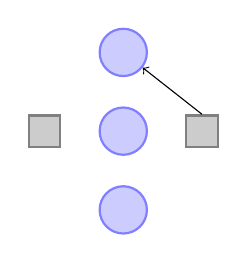
\begin{tikzpicture}
[place/.style={circle,draw=blue!50,fill=blue!20,thick,
inner sep=0pt,minimum size=6mm},
transition/.style={rectangle,draw=black!50,fill=black!20,thick,
inner sep=0pt,minimum size=4mm}]
\node at ( 0,2) [place] (waiting){};
\node at ( 0,1) [place] {};
\node at ( 0,0) [place] {};
\node at ( 1,1) [transition] (1){};
\node at (-1,1) [transition] {};
\draw [->] (1.north) -- (waiting);
\end{tikzpicture}
\end{center}

\subsection*{Klient}
\setlength{\unitlength}{4144sp}%
%
\begingroup\makeatletter\ifx\SetFigFont\undefined%
\gdef\SetFigFont#1#2#3#4#5{%
  \reset@font\fontsize{#1}{#2pt}%
  \fontfamily{#3}\fontseries{#4}\fontshape{#5}%
  \selectfont}%
\fi\endgroup%
\begin{picture}(1207,1568)(1830,-2083)
\put(1845,-689){\makebox(0,0)[lb]{\smash{{\SetFigFont{12}{14.4}{\rmdefault}{\mddefault}{\updefault}{\color[rgb]{0,0,0}+-----+}}}}}

\end{picture}%
\subsection*{Server}
obrazek distribuovana architektura

+--------+\\
| Jabber |\\
| client |     +--------+\\
+--------+     |        |\\
    |          | Jabber |      +..................+\\
    +----------| server |      :                  :\\
               |        |      :                  :\\
               +--------+      :                  :\\
                   |           :     Internet     :\\
                   +-----------:                  :-----------+\\
                               :                  :           |\\
                               :                  :       +--------+\\
                               :                  :       |        |\\
                               :                  :       | Jabber |\\
                               +..................:       | server |--------+\\
                                                          |        |        |\\
                                                          +--------+    +--------+\\
                                                                        | Jabber |\\
                                                                        | client |\\
                                                                        +--------+ \\
\section{Knihovny}
Jabber je realizov�n jako otev?en� XML standart pro instant messaging form�t, proto existuje mnoho programovac�ch jazyk?, kter�m je pr�ce s n�m 
usnadn?na pomoc� knihovny. Mezi nejzn�m?j?� pat?� C (iksemel, libstrophe, Loudmoutn), C++ (gloox, Iris), JAVA (JabberBeans, Smack, JSO, Feridian, Emite, minijingle), 
.NET (Jabber-Net, agsXMPP SDK), Python (JabberPy, PyXMPP, SleekXMPP, Twisted Words), Ruby (XMPP4R, Jabber4R, Jabber::Simple, Jabber::Bot), 
Perl (Net-Jabber) n?kter� n�?e budou lehce rozebr�ny a vyzdvi?eny jejich hlavn� p?ednosti.
\subsection*{iksemel}
\subsection*{JabberBeans}
\subsection*{Jabber-Net}


\subsection*{JabberPy}


\chapter{Dataming}
% \begin{tikzpicture}
% \pgftransformxscale{1.000000}
% \pgftransformyscale{-1.000000}
% \definecolor{dialinecolor}{rgb}{0.000000, 0.000000, 0.000000}
% \pgfsetstrokecolor{dialinecolor}
% \definecolor{dialinecolor}{rgb}{1.000000, 1.000000, 1.000000}
% \pgfsetfillcolor{dialinecolor}
% \pgfsetlinewidth{0.100000\du}
% \pgfsetdash{}{0pt}
% \definecolor{dialinecolor}{rgb}{1.000000, 1.000000, 1.000000}
% \pgfsetfillcolor{dialinecolor}
% \fill (0.568850\du,-138.031250\du)--(0.568850\du,-136.631250\du)--(8.383850\du,-136.631250\du)--(8.383850\du,-138.031250\du)--cycle;
% \definecolor{dialinecolor}{rgb}{0.000000, 0.000000, 0.000000}
% \pgfsetstrokecolor{dialinecolor}
% \draw (0.568850\du,-138.031250\du)--(0.568850\du,-136.631250\du)--(8.383850\du,-136.631250\du)--(8.383850\du,-138.031250\du)--cycle;
% % setfont left to latex
% \definecolor{dialinecolor}{rgb}{0.000000, 0.000000, 0.000000}
% \pgfsetstrokecolor{dialinecolor}
% \node at (4.476350\du,-137.081250\du){debug};
% \definecolor{dialinecolor}{rgb}{1.000000, 1.000000, 1.000000}
% \pgfsetfillcolor{dialinecolor}
% \fill (0.568850\du,-136.631250\du)--(0.568850\du,-132.431250\du)--(8.383850\du,-132.431250\du)--(8.383850\du,-136.631250\du)--cycle;
% \definecolor{dialinecolor}{rgb}{0.000000, 0.000000, 0.000000}
% \pgfsetstrokecolor{dialinecolor}
% \draw (0.568850\du,-136.631250\du)--(0.568850\du,-132.431250\du)--(8.383850\du,-132.431250\du)--(8.383850\du,-136.631250\du)--cycle;
% % setfont left to latex
% \definecolor{dialinecolor}{rgb}{0.000000, 0.000000, 0.000000}
% \pgfsetstrokecolor{dialinecolor}
% \node[anchor=west] at (0.718850\du,-135.931250\du){+id: serial};
% % setfont left to latex
% \definecolor{dialinecolor}{rgb}{0.000000, 0.000000, 0.000000}
% \pgfsetstrokecolor{dialinecolor}
% \node[anchor=west] at (0.718850\du,-135.131250\du){+area: integer};
% % setfont left to latex
% \definecolor{dialinecolor}{rgb}{0.000000, 0.000000, 0.000000}
% \pgfsetstrokecolor{dialinecolor}
% \node[anchor=west] at (0.718850\du,-134.331250\du){+dateadd: timestamp};
% % setfont left to latex
% \definecolor{dialinecolor}{rgb}{0.000000, 0.000000, 0.000000}
% \pgfsetstrokecolor{dialinecolor}
% \node[anchor=west] at (0.718850\du,-133.531250\du){+level: integer};
% % setfont left to latex
% \definecolor{dialinecolor}{rgb}{0.000000, 0.000000, 0.000000}
% \pgfsetstrokecolor{dialinecolor}
% \node[anchor=west] at (0.718850\du,-132.731250\du){+message: text};
% \pgfsetlinewidth{0.100000\du}
% \pgfsetdash{}{0pt}
% \definecolor{dialinecolor}{rgb}{1.000000, 1.000000, 1.000000}
% \pgfsetfillcolor{dialinecolor}
% \fill (10.568850\du,-138.006250\du)--(10.568850\du,-136.606250\du)--(18.768850\du,-136.606250\du)--(18.768850\du,-138.006250\du)--cycle;
% \definecolor{dialinecolor}{rgb}{0.000000, 0.000000, 0.000000}
% \pgfsetstrokecolor{dialinecolor}
% \draw (10.568850\du,-138.006250\du)--(10.568850\du,-136.606250\du)--(18.768850\du,-136.606250\du)--(18.768850\du,-138.006250\du)--cycle;
% % setfont left to latex
% \definecolor{dialinecolor}{rgb}{0.000000, 0.000000, 0.000000}
% \pgfsetstrokecolor{dialinecolor}
% \node at (14.668850\du,-137.056250\du){level};
% \definecolor{dialinecolor}{rgb}{1.000000, 1.000000, 1.000000}
% \pgfsetfillcolor{dialinecolor}
% \fill (10.568850\du,-136.606250\du)--(10.568850\du,-133.206250\du)--(18.768850\du,-133.206250\du)--(18.768850\du,-136.606250\du)--cycle;
% \definecolor{dialinecolor}{rgb}{0.000000, 0.000000, 0.000000}
% \pgfsetstrokecolor{dialinecolor}
% \draw (10.568850\du,-136.606250\du)--(10.568850\du,-133.206250\du)--(18.768850\du,-133.206250\du)--(18.768850\du,-136.606250\du)--cycle;
% % setfont left to latex
% \definecolor{dialinecolor}{rgb}{0.000000, 0.000000, 0.000000}
% \pgfsetstrokecolor{dialinecolor}
% \node[anchor=west] at (10.718850\du,-135.906250\du){+num: integer};
% % setfont left to latex
% \definecolor{dialinecolor}{rgb}{0.000000, 0.000000, 0.000000}
% \pgfsetstrokecolor{dialinecolor}
% \node[anchor=west] at (10.718850\du,-135.106250\du){+name: text};
% % setfont left to latex
% \definecolor{dialinecolor}{rgb}{0.000000, 0.000000, 0.000000}
% \pgfsetstrokecolor{dialinecolor}
% \node[anchor=west] at (10.718850\du,-134.306250\du){+description: text};
% % setfont left to latex
% \definecolor{dialinecolor}{rgb}{0.000000, 0.000000, 0.000000}
% \pgfsetstrokecolor{dialinecolor}
% \node[anchor=west] at (10.718850\du,-133.506250\du){+descriptioncz: text};
% \pgfsetlinewidth{0.100000\du}
% \pgfsetdash{}{0pt}
% \definecolor{dialinecolor}{rgb}{1.000000, 1.000000, 1.000000}
% \pgfsetfillcolor{dialinecolor}
% \fill (0.218950\du,-119.668750\du)--(0.218950\du,-118.268750\du)--(8.418950\du,-118.268750\du)--(8.418950\du,-119.668750\du)--cycle;
% \definecolor{dialinecolor}{rgb}{0.000000, 0.000000, 0.000000}
% \pgfsetstrokecolor{dialinecolor}
% \draw (0.218950\du,-119.668750\du)--(0.218950\du,-118.268750\du)--(8.418950\du,-118.268750\du)--(8.418950\du,-119.668750\du)--cycle;
% % setfont left to latex
% \definecolor{dialinecolor}{rgb}{0.000000, 0.000000, 0.000000}
% \pgfsetstrokecolor{dialinecolor}
% \node at (4.318950\du,-118.718750\du){logarea};
% \definecolor{dialinecolor}{rgb}{1.000000, 1.000000, 1.000000}
% \pgfsetfillcolor{dialinecolor}
% \fill (0.218950\du,-118.268750\du)--(0.218950\du,-114.868750\du)--(8.418950\du,-114.868750\du)--(8.418950\du,-118.268750\du)--cycle;
% \definecolor{dialinecolor}{rgb}{0.000000, 0.000000, 0.000000}
% \pgfsetstrokecolor{dialinecolor}
% \draw (0.218950\du,-118.268750\du)--(0.218950\du,-114.868750\du)--(8.418950\du,-114.868750\du)--(8.418950\du,-118.268750\du)--cycle;
% % setfont left to latex
% \definecolor{dialinecolor}{rgb}{0.000000, 0.000000, 0.000000}
% \pgfsetstrokecolor{dialinecolor}
% \node[anchor=west] at (0.368950\du,-117.568750\du){+num: serial};
% % setfont left to latex
% \definecolor{dialinecolor}{rgb}{0.000000, 0.000000, 0.000000}
% \pgfsetstrokecolor{dialinecolor}
% \node[anchor=west] at (0.368950\du,-116.768750\du){+name: text};
% % setfont left to latex
% \definecolor{dialinecolor}{rgb}{0.000000, 0.000000, 0.000000}
% \pgfsetstrokecolor{dialinecolor}
% \node[anchor=west] at (0.368950\du,-115.968750\du){+description: text};
% % setfont left to latex
% \definecolor{dialinecolor}{rgb}{0.000000, 0.000000, 0.000000}
% \pgfsetstrokecolor{dialinecolor}
% \node[anchor=west] at (0.368950\du,-115.168750\du){+descriptioncz: text};
% \pgfsetlinewidth{0.100000\du}
% \pgfsetdash{}{0pt}
% \definecolor{dialinecolor}{rgb}{1.000000, 1.000000, 1.000000}
% \pgfsetfillcolor{dialinecolor}
% \fill (1.068950\du,-130.018750\du)--(1.068950\du,-128.618750\du)--(7.728950\du,-128.618750\du)--(7.728950\du,-130.018750\du)--cycle;
% \definecolor{dialinecolor}{rgb}{0.000000, 0.000000, 0.000000}
% \pgfsetstrokecolor{dialinecolor}
% \draw (1.068950\du,-130.018750\du)--(1.068950\du,-128.618750\du)--(7.728950\du,-128.618750\du)--(7.728950\du,-130.018750\du)--cycle;
% % setfont left to latex
% \definecolor{dialinecolor}{rgb}{0.000000, 0.000000, 0.000000}
% \pgfsetstrokecolor{dialinecolor}
% \node at (4.398950\du,-129.068750\du){message};
% \definecolor{dialinecolor}{rgb}{1.000000, 1.000000, 1.000000}
% \pgfsetfillcolor{dialinecolor}
% \fill (1.068950\du,-128.618750\du)--(1.068950\du,-122.018750\du)--(7.728950\du,-122.018750\du)--(7.728950\du,-128.618750\du)--cycle;
% \definecolor{dialinecolor}{rgb}{0.000000, 0.000000, 0.000000}
% \pgfsetstrokecolor{dialinecolor}
% \draw (1.068950\du,-128.618750\du)--(1.068950\du,-122.018750\du)--(7.728950\du,-122.018750\du)--(7.728950\du,-128.618750\du)--cycle;
% % setfont left to latex
% \definecolor{dialinecolor}{rgb}{0.000000, 0.000000, 0.000000}
% \pgfsetstrokecolor{dialinecolor}
% \node[anchor=west] at (1.218950\du,-127.918750\du){+id: serial};
% % setfont left to latex
% \definecolor{dialinecolor}{rgb}{0.000000, 0.000000, 0.000000}
% \pgfsetstrokecolor{dialinecolor}
% \node[anchor=west] at (1.218950\du,-127.118750\du){+date: timestamp};
% % setfont left to latex
% \definecolor{dialinecolor}{rgb}{0.000000, 0.000000, 0.000000}
% \pgfsetstrokecolor{dialinecolor}
% \node[anchor=west] at (1.218950\du,-126.318750\du){+fromj: text};
% % setfont left to latex
% \definecolor{dialinecolor}{rgb}{0.000000, 0.000000, 0.000000}
% \pgfsetstrokecolor{dialinecolor}
% \node[anchor=west] at (1.218950\du,-125.518750\du){+toj: text};
% % setfont left to latex
% \definecolor{dialinecolor}{rgb}{0.000000, 0.000000, 0.000000}
% \pgfsetstrokecolor{dialinecolor}
% \node[anchor=west] at (1.218950\du,-124.718750\du){+message: text};
% % setfont left to latex
% \definecolor{dialinecolor}{rgb}{0.000000, 0.000000, 0.000000}
% \pgfsetstrokecolor{dialinecolor}
% \node[anchor=west] at (1.218950\du,-123.918750\du){+subject: text};
% % setfont left to latex
% \definecolor{dialinecolor}{rgb}{0.000000, 0.000000, 0.000000}
% \pgfsetstrokecolor{dialinecolor}
% \node[anchor=west] at (1.218950\du,-123.118750\du){+thread: text};
% % setfont left to latex
% \definecolor{dialinecolor}{rgb}{0.000000, 0.000000, 0.000000}
% \pgfsetstrokecolor{dialinecolor}
% \node[anchor=west] at (1.218950\du,-122.318750\du){+subtype: text};
% \pgfsetlinewidth{0.100000\du}
% \pgfsetdash{}{0pt}
% \definecolor{dialinecolor}{rgb}{1.000000, 1.000000, 1.000000}
% \pgfsetfillcolor{dialinecolor}
% \fill (11.018950\du,-130.918750\du)--(11.018950\du,-129.518750\du)--(18.448950\du,-129.518750\du)--(18.448950\du,-130.918750\du)--cycle;
% \definecolor{dialinecolor}{rgb}{0.000000, 0.000000, 0.000000}
% \pgfsetstrokecolor{dialinecolor}
% \draw (11.018950\du,-130.918750\du)--(11.018950\du,-129.518750\du)--(18.448950\du,-129.518750\du)--(18.448950\du,-130.918750\du)--cycle;
% % setfont left to latex
% \definecolor{dialinecolor}{rgb}{0.000000, 0.000000, 0.000000}
% \pgfsetstrokecolor{dialinecolor}
% \node at (14.733950\du,-129.968750\du){presence};
% \definecolor{dialinecolor}{rgb}{1.000000, 1.000000, 1.000000}
% \pgfsetfillcolor{dialinecolor}
% \fill (11.018950\du,-129.518750\du)--(11.018950\du,-121.318750\du)--(18.448950\du,-121.318750\du)--(18.448950\du,-129.518750\du)--cycle;
% \definecolor{dialinecolor}{rgb}{0.000000, 0.000000, 0.000000}
% \pgfsetstrokecolor{dialinecolor}
% \draw (11.018950\du,-129.518750\du)--(11.018950\du,-121.318750\du)--(18.448950\du,-121.318750\du)--(18.448950\du,-129.518750\du)--cycle;
% % setfont left to latex
% \definecolor{dialinecolor}{rgb}{0.000000, 0.000000, 0.000000}
% \pgfsetstrokecolor{dialinecolor}
% \node[anchor=west] at (11.168950\du,-128.818750\du){+id: serial};
% % setfont left to latex
% \definecolor{dialinecolor}{rgb}{0.000000, 0.000000, 0.000000}
% \pgfsetstrokecolor{dialinecolor}
% \node[anchor=west] at (11.168950\du,-128.018750\du){+date: timestamp};
% % setfont left to latex
% \definecolor{dialinecolor}{rgb}{0.000000, 0.000000, 0.000000}
% \pgfsetstrokecolor{dialinecolor}
% \node[anchor=west] at (11.168950\du,-127.218750\du){+fromj: text};
% % setfont left to latex
% \definecolor{dialinecolor}{rgb}{0.000000, 0.000000, 0.000000}
% \pgfsetstrokecolor{dialinecolor}
% \node[anchor=west] at (11.168950\du,-126.418750\du){+to: text};
% % setfont left to latex
% \definecolor{dialinecolor}{rgb}{0.000000, 0.000000, 0.000000}
% \pgfsetstrokecolor{dialinecolor}
% \node[anchor=west] at (11.168950\du,-125.618750\du){+message: text};
% % setfont left to latex
% \definecolor{dialinecolor}{rgb}{0.000000, 0.000000, 0.000000}
% \pgfsetstrokecolor{dialinecolor}
% \node[anchor=west] at (11.168950\du,-124.818750\du){+name: text};
% % setfont left to latex
% \definecolor{dialinecolor}{rgb}{0.000000, 0.000000, 0.000000}
% \pgfsetstrokecolor{dialinecolor}
% \node[anchor=west] at (11.168950\du,-124.018750\du){+resource: text};
% % setfont left to latex
% \definecolor{dialinecolor}{rgb}{0.000000, 0.000000, 0.000000}
% \pgfsetstrokecolor{dialinecolor}
% \node[anchor=west] at (11.168950\du,-123.218750\du){+presence: text};
% % setfont left to latex
% \definecolor{dialinecolor}{rgb}{0.000000, 0.000000, 0.000000}
% \pgfsetstrokecolor{dialinecolor}
% \node[anchor=west] at (11.168950\du,-122.418750\du){+status: text};
% % setfont left to latex
% \definecolor{dialinecolor}{rgb}{0.000000, 0.000000, 0.000000}
% \pgfsetstrokecolor{dialinecolor}
% \node[anchor=west] at (11.168950\du,-121.618750\du){+priority: integer};
% \pgfsetlinewidth{0.100000\du}
% \pgfsetdash{}{0pt}
% \definecolor{dialinecolor}{rgb}{1.000000, 1.000000, 1.000000}
% \pgfsetfillcolor{dialinecolor}
% \fill (-8.831050\du,-118.118750\du)--(-8.831050\du,-116.718750\du)--(-2.171050\du,-116.718750\du)--(-2.171050\du,-118.118750\du)--cycle;
% \definecolor{dialinecolor}{rgb}{0.000000, 0.000000, 0.000000}
% \pgfsetstrokecolor{dialinecolor}
% \draw (-8.831050\du,-118.118750\du)--(-8.831050\du,-116.718750\du)--(-2.171050\du,-116.718750\du)--(-2.171050\du,-118.118750\du)--cycle;
% % setfont left to latex
% \definecolor{dialinecolor}{rgb}{0.000000, 0.000000, 0.000000}
% \pgfsetstrokecolor{dialinecolor}
% \node at (-5.501050\du,-117.168750\du){userjid};
% \definecolor{dialinecolor}{rgb}{1.000000, 1.000000, 1.000000}
% \pgfsetfillcolor{dialinecolor}
% \fill (-8.831050\du,-116.718750\du)--(-8.831050\du,-114.918750\du)--(-2.171050\du,-114.918750\du)--(-2.171050\du,-116.718750\du)--cycle;
% \definecolor{dialinecolor}{rgb}{0.000000, 0.000000, 0.000000}
% \pgfsetstrokecolor{dialinecolor}
% \draw (-8.831050\du,-116.718750\du)--(-8.831050\du,-114.918750\du)--(-2.171050\du,-114.918750\du)--(-2.171050\du,-116.718750\du)--cycle;
% % setfont left to latex
% \definecolor{dialinecolor}{rgb}{0.000000, 0.000000, 0.000000}
% \pgfsetstrokecolor{dialinecolor}
% \node[anchor=west] at (-8.681050\du,-116.018750\du){+jidbare: text};
% % setfont left to latex
% \definecolor{dialinecolor}{rgb}{0.000000, 0.000000, 0.000000}
% \pgfsetstrokecolor{dialinecolor}
% \node[anchor=west] at (-8.681050\du,-115.218750\du){+date: timestamp};
% \pgfsetlinewidth{0.100000\du}
% \pgfsetdash{}{0pt}
% \definecolor{dialinecolor}{rgb}{1.000000, 1.000000, 1.000000}
% \pgfsetfillcolor{dialinecolor}
% \fill (-9.431050\du,-138.018750\du)--(-9.431050\du,-136.618750\du)--(-1.616050\du,-136.618750\du)--(-1.616050\du,-138.018750\du)--cycle;
% \definecolor{dialinecolor}{rgb}{0.000000, 0.000000, 0.000000}
% \pgfsetstrokecolor{dialinecolor}
% \draw (-9.431050\du,-138.018750\du)--(-9.431050\du,-136.618750\du)--(-1.616050\du,-136.618750\du)--(-1.616050\du,-138.018750\du)--cycle;
% % setfont left to latex
% \definecolor{dialinecolor}{rgb}{0.000000, 0.000000, 0.000000}
% \pgfsetstrokecolor{dialinecolor}
% \node at (-5.523550\du,-137.068750\du){vcard};
% \definecolor{dialinecolor}{rgb}{1.000000, 1.000000, 1.000000}
% \pgfsetfillcolor{dialinecolor}
% \fill (-9.431050\du,-136.618750\du)--(-9.431050\du,-119.618750\du)--(-1.616050\du,-119.618750\du)--(-1.616050\du,-136.618750\du)--cycle;
% \definecolor{dialinecolor}{rgb}{0.000000, 0.000000, 0.000000}
% \pgfsetstrokecolor{dialinecolor}
% \draw (-9.431050\du,-136.618750\du)--(-9.431050\du,-119.618750\du)--(-1.616050\du,-119.618750\du)--(-1.616050\du,-136.618750\du)--cycle;
% % setfont left to latex
% \definecolor{dialinecolor}{rgb}{0.000000, 0.000000, 0.000000}
% \pgfsetstrokecolor{dialinecolor}
% \node[anchor=west] at (-9.281050\du,-135.918750\du){+id: serial};
% % setfont left to latex
% \definecolor{dialinecolor}{rgb}{0.000000, 0.000000, 0.000000}
% \pgfsetstrokecolor{dialinecolor}
% \node[anchor=west] at (-9.281050\du,-135.118750\du){+jid: text};
% % setfont left to latex
% \definecolor{dialinecolor}{rgb}{0.000000, 0.000000, 0.000000}
% \pgfsetstrokecolor{dialinecolor}
% \node[anchor=west] at (-9.281050\du,-134.318750\du){+dateadd: timestamp};
% % setfont left to latex
% \definecolor{dialinecolor}{rgb}{0.000000, 0.000000, 0.000000}
% \pgfsetstrokecolor{dialinecolor}
% \node[anchor=west] at (-9.281050\du,-133.518750\du){+family: text};
% % setfont left to latex
% \definecolor{dialinecolor}{rgb}{0.000000, 0.000000, 0.000000}
% \pgfsetstrokecolor{dialinecolor}
% \node[anchor=west] at (-9.281050\du,-132.718750\du){+given: text};
% % setfont left to latex
% \definecolor{dialinecolor}{rgb}{0.000000, 0.000000, 0.000000}
% \pgfsetstrokecolor{dialinecolor}
% \node[anchor=west] at (-9.281050\du,-131.918750\du){+middle: text};
% % setfont left to latex
% \definecolor{dialinecolor}{rgb}{0.000000, 0.000000, 0.000000}
% \pgfsetstrokecolor{dialinecolor}
% \node[anchor=west] at (-9.281050\du,-131.118750\du){+prefix: text};
% % setfont left to latex
% \definecolor{dialinecolor}{rgb}{0.000000, 0.000000, 0.000000}
% \pgfsetstrokecolor{dialinecolor}
% \node[anchor=west] at (-9.281050\du,-130.318750\du){+suffix: text};
% % setfont left to latex
% \definecolor{dialinecolor}{rgb}{0.000000, 0.000000, 0.000000}
% \pgfsetstrokecolor{dialinecolor}
% \node[anchor=west] at (-9.281050\du,-129.518750\du){+nickname: text};
% % setfont left to latex
% \definecolor{dialinecolor}{rgb}{0.000000, 0.000000, 0.000000}
% \pgfsetstrokecolor{dialinecolor}
% \node[anchor=west] at (-9.281050\du,-128.718750\du){+url: text};
% % setfont left to latex
% \definecolor{dialinecolor}{rgb}{0.000000, 0.000000, 0.000000}
% \pgfsetstrokecolor{dialinecolor}
% \node[anchor=west] at (-9.281050\du,-127.918750\du){+bday: text};
% % setfont left to latex
% \definecolor{dialinecolor}{rgb}{0.000000, 0.000000, 0.000000}
% \pgfsetstrokecolor{dialinecolor}
% \node[anchor=west] at (-9.281050\du,-127.118750\du){+jabberid: text};
% % setfont left to latex
% \definecolor{dialinecolor}{rgb}{0.000000, 0.000000, 0.000000}
% \pgfsetstrokecolor{dialinecolor}
% \node[anchor=west] at (-9.281050\du,-126.318750\du){+title: text};
% % setfont left to latex
% \definecolor{dialinecolor}{rgb}{0.000000, 0.000000, 0.000000}
% \pgfsetstrokecolor{dialinecolor}
% \node[anchor=west] at (-9.281050\du,-125.518750\du){+role: text};
% % setfont left to latex
% \definecolor{dialinecolor}{rgb}{0.000000, 0.000000, 0.000000}
% \pgfsetstrokecolor{dialinecolor}
% \node[anchor=west] at (-9.281050\du,-124.718750\du){+note: text};
% % setfont left to latex
% \definecolor{dialinecolor}{rgb}{0.000000, 0.000000, 0.000000}
% \pgfsetstrokecolor{dialinecolor}
% \node[anchor=west] at (-9.281050\du,-123.918750\du){+mailer: text};
% % setfont left to latex
% \definecolor{dialinecolor}{rgb}{0.000000, 0.000000, 0.000000}
% \pgfsetstrokecolor{dialinecolor}
% \node[anchor=west] at (-9.281050\du,-123.118750\du){+rev: text};
% % setfont left to latex
% \definecolor{dialinecolor}{rgb}{0.000000, 0.000000, 0.000000}
% \pgfsetstrokecolor{dialinecolor}
% \node[anchor=west] at (-9.281050\du,-122.318750\du){+uid: text};
% % setfont left to latex
% \definecolor{dialinecolor}{rgb}{0.000000, 0.000000, 0.000000}
% \pgfsetstrokecolor{dialinecolor}
% \node[anchor=west] at (-9.281050\du,-121.518750\du){+tz: text};
% % setfont left to latex
% \definecolor{dialinecolor}{rgb}{0.000000, 0.000000, 0.000000}
% \pgfsetstrokecolor{dialinecolor}
% \node[anchor=west] at (-9.281050\du,-120.718750\du){+prodid: text};
% % setfont left to latex
% \definecolor{dialinecolor}{rgb}{0.000000, 0.000000, 0.000000}
% \pgfsetstrokecolor{dialinecolor}
% \node[anchor=west] at (-9.281050\du,-119.918750\du){+sotstring: text};
% \pgfsetlinewidth{0.100000\du}
% \pgfsetdash{}{0pt}
% \definecolor{dialinecolor}{rgb}{1.000000, 1.000000, 1.000000}
% \pgfsetfillcolor{dialinecolor}
% \fill (11.093950\du,-119.693750\du)--(11.093950\du,-118.293750\du)--(18.908950\du,-118.293750\du)--(18.908950\du,-119.693750\du)--cycle;
% \definecolor{dialinecolor}{rgb}{0.000000, 0.000000, 0.000000}
% \pgfsetstrokecolor{dialinecolor}
% \draw (11.093950\du,-119.693750\du)--(11.093950\du,-118.293750\du)--(18.908950\du,-118.293750\du)--(18.908950\du,-119.693750\du)--cycle;
% % setfont left to latex
% \definecolor{dialinecolor}{rgb}{0.000000, 0.000000, 0.000000}
% \pgfsetstrokecolor{dialinecolor}
% \node at (15.001450\du,-118.743750\du){xml};
% \definecolor{dialinecolor}{rgb}{1.000000, 1.000000, 1.000000}
% \pgfsetfillcolor{dialinecolor}
% \fill (11.093950\du,-118.293750\du)--(11.093950\du,-114.093750\du)--(18.908950\du,-114.093750\du)--(18.908950\du,-118.293750\du)--cycle;
% \definecolor{dialinecolor}{rgb}{0.000000, 0.000000, 0.000000}
% \pgfsetstrokecolor{dialinecolor}
% \draw (11.093950\du,-118.293750\du)--(11.093950\du,-114.093750\du)--(18.908950\du,-114.093750\du)--(18.908950\du,-118.293750\du)--cycle;
% % setfont left to latex
% \definecolor{dialinecolor}{rgb}{0.000000, 0.000000, 0.000000}
% \pgfsetstrokecolor{dialinecolor}
% \node[anchor=west] at (11.243950\du,-117.593750\du){+id: serial};
% % setfont left to latex
% \definecolor{dialinecolor}{rgb}{0.000000, 0.000000, 0.000000}
% \pgfsetstrokecolor{dialinecolor}
% \node[anchor=west] at (11.243950\du,-116.793750\du){+area: integer};
% % setfont left to latex
% \definecolor{dialinecolor}{rgb}{0.000000, 0.000000, 0.000000}
% \pgfsetstrokecolor{dialinecolor}
% \node[anchor=west] at (11.243950\du,-115.993750\du){+dateadd: timestamp};
% % setfont left to latex
% \definecolor{dialinecolor}{rgb}{0.000000, 0.000000, 0.000000}
% \pgfsetstrokecolor{dialinecolor}
% \node[anchor=west] at (11.243950\du,-115.193750\du){+level: integer};
% % setfont left to latex
% \definecolor{dialinecolor}{rgb}{0.000000, 0.000000, 0.000000}
% \pgfsetstrokecolor{dialinecolor}
% \node[anchor=west] at (11.243950\du,-114.393750\du){+message: text};
% \end{tikzpicture}



\section{Metody dolovani dat}
\section{Dolovani znalosti z databazi}






\chapter{Developer}

\section{Cile}

\section{Slepa ulicka}

\section{knihivna, jazyk}

\section{Jine produkty}


\chapter{Nikdy to nebude naprosto dokonal�}


\chapter{Typografick� a~jazykov� z�sady}

\section{Co to je normovan� str�nka?}

\chapter{Z�v?r}
 % viz. obsah.tex

  % Pouzita literatura
  % ----------------------------------------------
\ifczech
  \bibliographystyle{czechiso}
\else 
  \bibliographystyle{plain}
%  \bibliographystyle{alpha}
\fi
  \begin{flushleft}
  \bibliography{literatura} % viz. literatura.bib
  \end{flushleft}
  \appendix
  
  \chapter{Obsah CD}
\begin{figure}[h]
\begin{verbatim}
./doc/                 - programov� dokumentace

./src/jabinfo          - zdrojov� soubory robota

./src/transformation   - zdrojov� soubory transformace

./src/datamining       - zdrojov� soubory data miningu

./tex/                 - zdrojov� data technick� zpr�vy

./www/                 - zdrojov� data webov� prezentace

./bp-xsendl00.pdf      - technick� zpr�va

./MANUAL               - manu�l k programu jabinfo

./README               - z�kladn� informace
\end{verbatim}
\end{figure} 

%\chapter{Manual}
%\chapter{Konfigra�n� soubor}
%\chapter{RelaxNG Sch�ma konfigura�n�ho soboru}
%\chapter{Plakat}

\chapter{Slovn�k zkratek}
\begin{description}
\item [Base64] --- p�eveden� bin�rn�ch dat pomoc� znak� ASCII.
\item [CSV] (Comma-separated values) --- souborov� form�t ur�en� pro v�m�nu dat z tabulek.
\item [GPG] (GNU Privacy Guard) --- slou�� k podepisov�n� a kontrolu podpisu r�zn�ch dat.
\item [ID3v1] --- datov� form�t obsahuj�c� informace o skladb�.
\item [IM slu�by] (Instant messaging) ---  umo��uj� pos�lat zpr�vy a komunikovat mezi u�ivateli.% a poskytuj� dal�� funkce. 
\item [Jabber] --- viz XMPP.
\item [JEP] (Jabber Enhancement Proposal) --- star�� n�zev pro XEP.
\item [JID] (Jabber ID) --- jednozna�n� identifik�tor v s�ti Jabber.
\item [SASL] (Simple Authentication and Security Layer) --- metoda slou��c� ov��ov�n� klient� na serverech.
\item [Stanza] --- XML stream.
\item [SQL] (Structured Query Language) ---  jazyk pou��van� pro komunikaci s datab�zemi.
\item [TLS] (Transport Layer Security) --- kryptografick� protokol, poskytuje zabezpe�enou komunikaci na internetu.
\item [TSQL] (Transact-SQL) --- jezyk pro tempor�ln� datab�ze.
\item [vCard] ---  elektronick� osobn� vizitka.
\item [XEP] (XMPP Extension Protocol) --- roz�i�uje protokol RFC.
\item [XML] (Extensible Markup Language) --- univerz�ln� zna�kovac� jazyk.
\item [XMPP] (Extensible Messaging and Presence Protocol) --- protokol pro doru�ov�n� zpr�v.
\end{description}

\chapter{Stanza - z�kladn� sch�ma}\label{Estanza}

P�ehled z�kladn�ch element�, kter� jsou vyu��v�ny p�i Jabber komunikaci. Struktura jednotliv�ch ��st� stanzy ukazuje pouze prvky relativn� k t�to pr�ci. Pomoc� hranat�ch z�vorek je zn�zorn�na mno�ina, ze kter� mus� b�t vybr�n pr�v� jeden prvek. Na m�st� uvozovek se o�ek�v� jak�koliv povolen� hodnota.


\section*{Iq}\label{Eiq}

\begin{figure}[h]
\lstset{language=Xml ,caption={Popis elementu \textit{iq}.},label=picEiq}
\begin{lstlisting}
          <iq from=""
              to=""
              type="[get,set,result,error]"
              id=""
            Namespace
          </iq>
\end{lstlisting}
\end{figure}

%\begin{table}[h]
%\begin{center}
%\begin{tabular}{ l  l  l  l } 
%jabber:client & jabber:server& jabber:iq:auth& jabber:iq:register\\ 
%jabber:iq:roster& jabber:x:offline& jabber:iq:agent& jabber:iq:agents\\ 
% jabber:x:delay& jabber:iq:version& jabber:iq:time& vcard-temp\\ 
% jabber:iq:private& jabber:iq:search& jabber:iq:oob& jabber:x:oob\\ 
% jabber:iq:admin& jabber:iq:filter& jabber:iq:auth:0k& jabber:iq:browse\\ 
%jabber:x:event& jabber:iq:conference& jabber:x:signed& jabber:x:encrypted\\ 
% jabber:iq:gateway& jabber:iq:last& jabber:x:envelope& jabber:x:expire\\ 	
%  jabber:xdb:ginsert& jabber:xdb:nslist&\multicolumn{2}{l}{texthttp://www.w3.org/1999/xhtml}
%\end{tabular}
%\caption{P�ehled Namespace elementu \textit{iq}.}
%\label{tabNamespaceIqE}
%\end{center} 
%\end{table}


\section*{Message}\label{Emessage}

\begin{figure}[h]
\lstset{language=Xml ,caption={Popis elementu \textit{message}.},label=picMessageE}
\begin{lstlisting}
      <message from=""
               to=""
               type="[normal,chat,groupchat, headline, error]"
               id=""
        <body>  </body>
        <x xmlns="jabber:x:event">
           [Offline, Delivered, Displayed, Composing]
        <subject>  </subject>
        <thread>   </thread>
        <error>    </error>
        <x>        </x>
      </message>
\end{lstlisting}
\end{figure}

\section*{Presence}\label{Epresence}

\begin{figure}[h]
\lstset{language=Xml ,caption={Popis elementu \textit{presence}.},label=picPresenceE}
\begin{lstlisting}
      <presence from=""
                to=""
                type="[available, unavailable, probe, subscribe,
                       unsubscribe, subscribed, unsubscribed, error]"
                id=""
        <show>
          [away, chat, dnd, normal, xa]
        </show>
        <status>     </status>
        <priority>   </priority>
        <error>      </error>
      </presence>
\end{lstlisting}
\end{figure}


\newpage
\section*{P�ehled pr�b�hu roz���en�}\label{Erozsireni}

Uk�zka cel�ho p��kladu ���en� statusu pomoc� roz���en� \textit{User Tune}. U�ivatel \textit{user} poslouch� hudbu a informuje server zasl�n�m zpr�vy zobrazen� v p��kladu \ref{picSPep1}.
\begin{figure}[h]
\begin{center}
% Graphic for TeX using PGF
% Title: /home/portilo/School/IPB/Text/Dia/stanza.dia
% Creator: Dia v0.97.1
% CreationDate: Tue Apr 19 00:48:17 2011
% For: portilo
% \usepackage{tikz}
% The following commands are not supported in PSTricks at present
% We define them conditionally, so when they are implemented,
% this pgf file will use them.
\ifx\du\undefined
  \newlength{\du}
\fi
\setlength{\du}{15\unitlength}
\begin{tikzpicture}
\pgftransformxscale{1.000000}
\pgftransformyscale{-1.000000}
\definecolor{dialinecolor}{rgb}{0.000000, 0.000000, 0.000000}
\pgfsetstrokecolor{dialinecolor}
\definecolor{dialinecolor}{rgb}{1.000000, 1.000000, 1.000000}
\pgfsetfillcolor{dialinecolor}
\pgfsetlinewidth{0.050000\du}
\pgfsetdash{}{0pt}
\pgfsetdash{}{0pt}
\pgfsetbuttcap
{
\definecolor{dialinecolor}{rgb}{0.000000, 0.000000, 0.000000}
\pgfsetfillcolor{dialinecolor}
% was here!!!
\definecolor{dialinecolor}{rgb}{0.000000, 0.000000, 0.000000}
\pgfsetstrokecolor{dialinecolor}
\draw (-2.525000\du,-17.387500\du)--(-2.523338\du,-5.093724\du);
}
% setfont left to latex
\definecolor{dialinecolor}{rgb}{0.000000, 0.000000, 0.000000}
\pgfsetstrokecolor{dialinecolor}
\node[anchor=west] at (-5.681338\du,-17.668724\du){user@jabbim.com};
% setfont left to latex
\definecolor{dialinecolor}{rgb}{0.000000, 0.000000, 0.000000}
\pgfsetstrokecolor{dialinecolor}
\node[anchor=west] at (4.157662\du,-17.693724\du){server};
% setfont left to latex
\definecolor{dialinecolor}{rgb}{0.000000, 0.000000, 0.000000}
\pgfsetstrokecolor{dialinecolor}
\node[anchor=west] at (11.626662\du,-18.530724\du){u�ivatel�};
% setfont left to latex
\definecolor{dialinecolor}{rgb}{0.000000, 0.000000, 0.000000}
\pgfsetstrokecolor{dialinecolor}
\node[anchor=west] at (11.126662\du,-17.730724\du){kontakt listu};
\pgfsetlinewidth{0.040000\du}
\pgfsetdash{{\pgflinewidth}{0.200000\du}}{0cm}
\pgfsetdash{{\pgflinewidth}{0.200000\du}}{0cm}
\pgfsetbuttcap
{
\definecolor{dialinecolor}{rgb}{0.000000, 0.000000, 0.000000}
\pgfsetfillcolor{dialinecolor}
% was here!!!
\pgfsetarrowsend{to}
\definecolor{dialinecolor}{rgb}{0.000000, 0.000000, 0.000000}
\pgfsetstrokecolor{dialinecolor}
\draw (-2.520597\du,-14.123984\du)--(5.381059\du,-13.197521\du);
}
% setfont left to latex
\definecolor{dialinecolor}{rgb}{0.000000, 0.000000, 0.000000}
\pgfsetstrokecolor{dialinecolor}
\node[anchor=west] at (-8.273338\du,-14.118724\du){};
\pgfsetlinewidth{0.050000\du}
\pgfsetdash{}{0pt}
\pgfsetdash{}{0pt}
\pgfsetbuttcap
{
\definecolor{dialinecolor}{rgb}{0.000000, 0.000000, 0.000000}
\pgfsetfillcolor{dialinecolor}
% was here!!!
\definecolor{dialinecolor}{rgb}{0.000000, 0.000000, 0.000000}
\pgfsetstrokecolor{dialinecolor}
\draw (5.337463\du,-17.388218\du)--(5.339125\du,-5.094442\du);
}
\pgfsetlinewidth{0.050000\du}
\pgfsetdash{}{0pt}
\pgfsetdash{}{0pt}
\pgfsetbuttcap
{
\definecolor{dialinecolor}{rgb}{0.000000, 0.000000, 0.000000}
\pgfsetfillcolor{dialinecolor}
% was here!!!
\definecolor{dialinecolor}{rgb}{0.000000, 0.000000, 0.000000}
\pgfsetstrokecolor{dialinecolor}
\draw (13.190563\du,-17.406418\du)--(13.192225\du,-5.112642\du);
}
\pgfsetlinewidth{0.040000\du}
\pgfsetdash{{\pgflinewidth}{0.200000\du}}{0cm}
\pgfsetdash{{\pgflinewidth}{0.200000\du}}{0cm}
\pgfsetbuttcap
{
\definecolor{dialinecolor}{rgb}{0.000000, 0.000000, 0.000000}
\pgfsetfillcolor{dialinecolor}
% was here!!!
\pgfsetarrowsend{to}
\definecolor{dialinecolor}{rgb}{0.000000, 0.000000, 0.000000}
\pgfsetstrokecolor{dialinecolor}
\draw (5.315252\du,-12.690528\du)--(13.216909\du,-11.764065\du);
}
\pgfsetlinewidth{0.040000\du}
\pgfsetdash{{\pgflinewidth}{0.200000\du}}{0cm}
\pgfsetdash{{\pgflinewidth}{0.200000\du}}{0cm}
\pgfsetbuttcap
{
\definecolor{dialinecolor}{rgb}{0.000000, 0.000000, 0.000000}
\pgfsetfillcolor{dialinecolor}
% was here!!!
\pgfsetarrowsend{to}
\definecolor{dialinecolor}{rgb}{0.000000, 0.000000, 0.000000}
\pgfsetstrokecolor{dialinecolor}
\draw (5.323252\du,-7.549728\du)--(13.224909\du,-6.623265\du);
}
\pgfsetlinewidth{0.040000\du}
\pgfsetdash{{\pgflinewidth}{0.200000\du}}{0cm}
\pgfsetdash{{\pgflinewidth}{0.200000\du}}{0cm}
\pgfsetbuttcap
{
\definecolor{dialinecolor}{rgb}{0.000000, 0.000000, 0.000000}
\pgfsetfillcolor{dialinecolor}
% was here!!!
\pgfsetarrowsend{to}
\definecolor{dialinecolor}{rgb}{0.000000, 0.000000, 0.000000}
\pgfsetstrokecolor{dialinecolor}
\draw (-2.524748\du,-9.480928\du)--(5.376909\du,-8.554465\du);
}
\pgfsetlinewidth{0.050000\du}
\pgfsetdash{}{0pt}
\pgfsetdash{}{0pt}
\pgfsetmiterjoin
\definecolor{dialinecolor}{rgb}{1.000000, 1.000000, 1.000000}
\pgfsetfillcolor{dialinecolor}
\fill (-0.778941\du,-14.433521\du)--(-0.778941\du,-12.849521\du)--(3.605059\du,-12.849521\du)--(3.605059\du,-14.433521\du)--cycle;
\definecolor{dialinecolor}{rgb}{0.000000, 0.000000, 0.000000}
\pgfsetstrokecolor{dialinecolor}
\draw (-0.778941\du,-14.433521\du)--(-0.778941\du,-12.849521\du)--(3.605059\du,-12.849521\du)--(3.605059\du,-14.433521\du)--cycle;
\pgfsetlinewidth{0.050000\du}
\pgfsetdash{}{0pt}
\pgfsetdash{}{0pt}
\pgfsetmiterjoin
\definecolor{dialinecolor}{rgb}{1.000000, 1.000000, 1.000000}
\pgfsetfillcolor{dialinecolor}
\fill (-0.777941\du,-9.715721\du)--(-0.777941\du,-8.131721\du)--(3.606059\du,-8.131721\du)--(3.606059\du,-9.715721\du)--cycle;
\definecolor{dialinecolor}{rgb}{0.000000, 0.000000, 0.000000}
\pgfsetstrokecolor{dialinecolor}
\draw (-0.777941\du,-9.715721\du)--(-0.777941\du,-8.131721\du)--(3.606059\du,-8.131721\du)--(3.606059\du,-9.715721\du)--cycle;
\pgfsetlinewidth{0.050000\du}
\pgfsetdash{}{0pt}
\pgfsetdash{}{0pt}
\pgfsetmiterjoin
\definecolor{dialinecolor}{rgb}{1.000000, 1.000000, 1.000000}
\pgfsetfillcolor{dialinecolor}
\fill (6.958059\du,-13.022921\du)--(6.958059\du,-11.438921\du)--(11.342059\du,-11.438921\du)--(11.342059\du,-13.022921\du)--cycle;
\definecolor{dialinecolor}{rgb}{0.000000, 0.000000, 0.000000}
\pgfsetstrokecolor{dialinecolor}
\draw (6.958059\du,-13.022921\du)--(6.958059\du,-11.438921\du)--(11.342059\du,-11.438921\du)--(11.342059\du,-13.022921\du)--cycle;
\pgfsetlinewidth{0.050000\du}
\pgfsetdash{}{0pt}
\pgfsetdash{}{0pt}
\pgfsetmiterjoin
\definecolor{dialinecolor}{rgb}{1.000000, 1.000000, 1.000000}
\pgfsetfillcolor{dialinecolor}
\fill (6.982059\du,-7.834121\du)--(6.982059\du,-6.250121\du)--(11.366059\du,-6.250121\du)--(11.366059\du,-7.834121\du)--cycle;
\definecolor{dialinecolor}{rgb}{0.000000, 0.000000, 0.000000}
\pgfsetstrokecolor{dialinecolor}
\draw (6.982059\du,-7.834121\du)--(6.982059\du,-6.250121\du)--(11.366059\du,-6.250121\du)--(11.366059\du,-7.834121\du)--cycle;
% setfont left to latex
\definecolor{dialinecolor}{rgb}{0.000000, 0.000000, 0.000000}
\pgfsetstrokecolor{dialinecolor}
\node[anchor=west] at (-0.602941\du,-13.593521\du){zpr�va \ref{picSPep1}};
% setfont left to latex
\definecolor{dialinecolor}{rgb}{0.000000, 0.000000, 0.000000}
\pgfsetstrokecolor{dialinecolor}
\node[anchor=west] at (-0.546941\du,-8.773721\du){zpr�va \ref{picSPep3}};
% setfont left to latex
\definecolor{dialinecolor}{rgb}{0.000000, 0.000000, 0.000000}
\pgfsetstrokecolor{dialinecolor}
\node[anchor=west] at (7.157059\du,-12.144921\du){zpr�va \ref{picSPep2}};
% setfont left to latex
\definecolor{dialinecolor}{rgb}{0.000000, 0.000000, 0.000000}
\pgfsetstrokecolor{dialinecolor}
\node[anchor=west] at (7.213059\du,-7.036121\du){zpr�va \ref{picSPep4}};
\end{tikzpicture}

\caption{Uk�zka \uv{���en�} \textit{User Tune}.}
 \label{dbscan}
\end{center}
\end{figure}

\begin{figure}[h]
\lstset{language=Xml ,caption={Informov�n� serveru o pr�v� p�ehr�vaj�c� hudb�.},label=picSPep1}
\begin{lstlisting}
      <iq from="user@jabbim.com" type="set" id="pub1">
         <pubsub xmlns="http://jabber.org/protocol/pubsub">
            <publish node="http://jabber.org/protocol/tune">
               <item>
                  <tune xmlns="http://jabber.org/protocol/tune">
                     <artist>Daniel Landa</artist>
                     <length>255</length>
                     <source>Nigredo</source>
                     <title>1968</title>
                     <track>5</track>
                  </tune>
               </item>
            </publish>
         </pubsub>
      </iq>
\end{lstlisting}
\end{figure}
\newpage
Server obdr�� informace od klienta \textit{user} zpr�vu o p�ehr�vaj�c� hudb�. Pomoc� elementu \textit{message} ji p�epo�le v�em u�ivatel�m z kontakt listu u�ivatele \textit{user}, kte�� jsou pro odb�r t�chto typ� zpr�v zaregistrov�ni. Tato struktura zpr�vy je prezentov�na na p��kladu \ref{picSPep2}.
\begin{figure}[h]
\lstset{language=Xml ,caption={Server informuje u�ivatele podporuj�c� roz���en� o stavu \textit{user@jabbim.com}.},label=picSPep2}
\begin{lstlisting}
      <message from="user@jabbim.com" type="set"
               to="jabinfo@jabbim.com/bot" id="pub1">
         <event xmlns="http://jabber.org/protocol/pubsub#event">
            <items node="http://jabber.org/protocol/tune">
               <item>
                  <tune xmlns="http://jabber.org/protocol/tune">
                     <artist>Daniel Landa</artist>
                     <length>255</length>
                     <source>Nigredo</source>
                     <title>1968</title>
                    <track>5</track>
                  </tune>
               </item>
            </items>
         </event>
      </message>
\end{lstlisting}
\end{figure}

Zpr�va o p�ehr�van� hudb� je tak� p�eposl�na v�em otev�en�m spojen�m u�ivatele \textit{user}, uk�z�no na p��klad� \ref{picSPep3}.

\begin{figure}[h]
\lstset{language=Xml ,caption={Server p�epo�le informace o p�ehr�van� hudb� v�em otev�en�m spojen�m u�ivatele \textit{user@jabbim.com}.},label=picSPep3}
\begin{lstlisting}
      <message from="user@jabbim.com" type="set"
               to="user@jabbim.com/doma" id="pub2">
         <event xmlns="http://jabber.org/protocol/pubsub#event">
            <items node="http://jabber.org/protocol/tune">
               <item>
                  <tune xmlns="http://jabber.org/protocol/tune">
                     <artist>Daniel Landa</artist>
                     <length>255</length>
                     <source>Nigredo</source>
                     <title>1968</title>
                     <track>5</track>
                  </tune>
               </item>
            </items>
         </event>
      </message>
\end{lstlisting}
\end{figure}
\newpage
P�estane--li u�ivatel \textit{user} poslouchat/vys�lat informace o p�ehr�van� hudb�, provede to pomoc� zpr�vy uk�zan� na p��kladu \ref{picSPep4}. Zpr�va typu \textit{iq}, ve kter� je polo�ka \textit{tune} nesouc� informace o skladb� pr�zdn�.
\begin{figure}[h]
\lstset{language=Xml ,caption={U�ivatel ukon�il \uv{vys�lan�} roz���en�ch zpr�v o sv�m stavu.},label=picSPep4}
\begin{lstlisting}
      <iq from="user@jabbim.com/prace" type="set" id="pub1">
         <pubsub xmlns="http://jabber.org/protocol/pubsub">
            <publish node="http://jabber.org/protocol/tune">
               <item>
                  <tune xmlns="http://jabber.org/protocol/tune"/>
               </item>
            </publish>
         </pubsub>
      </iq>
\end{lstlisting}
\end{figure}

Server informuje v�echny ��astn�ky odb�ru zpr�vou, kter� m� polo�ku \textit{tune} pr�zdnou. Tak jak to prezentuje p��klad \ref{picSPep5}.

\begin{figure}[h]
\lstset{language=Xml ,caption={Server informuje klienty o ukon�en� ���en� roz���en�ho statusu.},label=picSPep5}
\begin{lstlisting}
      <message from="user@jabbim.com"
               to="jabinfo@jabbim.com/bot">
         <event xmlns="http://jabber.org/protocol/pubsub#event">
            <items node="http://jabber.org/protocol/tune">
               <item>
                  <tune xmlns="http://jabber.org/protocol/tune"/>
               </item>
            </items>
         </event>
      </message>
\end{lstlisting}
\end{figure}

\chapter{N�vrh datab�ze}\label{EDatabase}

\begin{figure}[ht]
\begin{center}
% Graphic for TeX using PGF
% Title: /home/portilo/School/IPB/Text/Dia/Database.dia
% Creator: Dia v0.97.1
% CreationDate: Thu Apr 14 23:14:16 2011
% For: portilo
% \usepackage{tikz}
% The following commands are not supported in PSTricks at present
% We define them conditionally, so when they are implemented,
% this pgf file will use them.
\ifx\du\undefined
  \newlength{\du}
\fi
\setlength{\du}{15\unitlength}
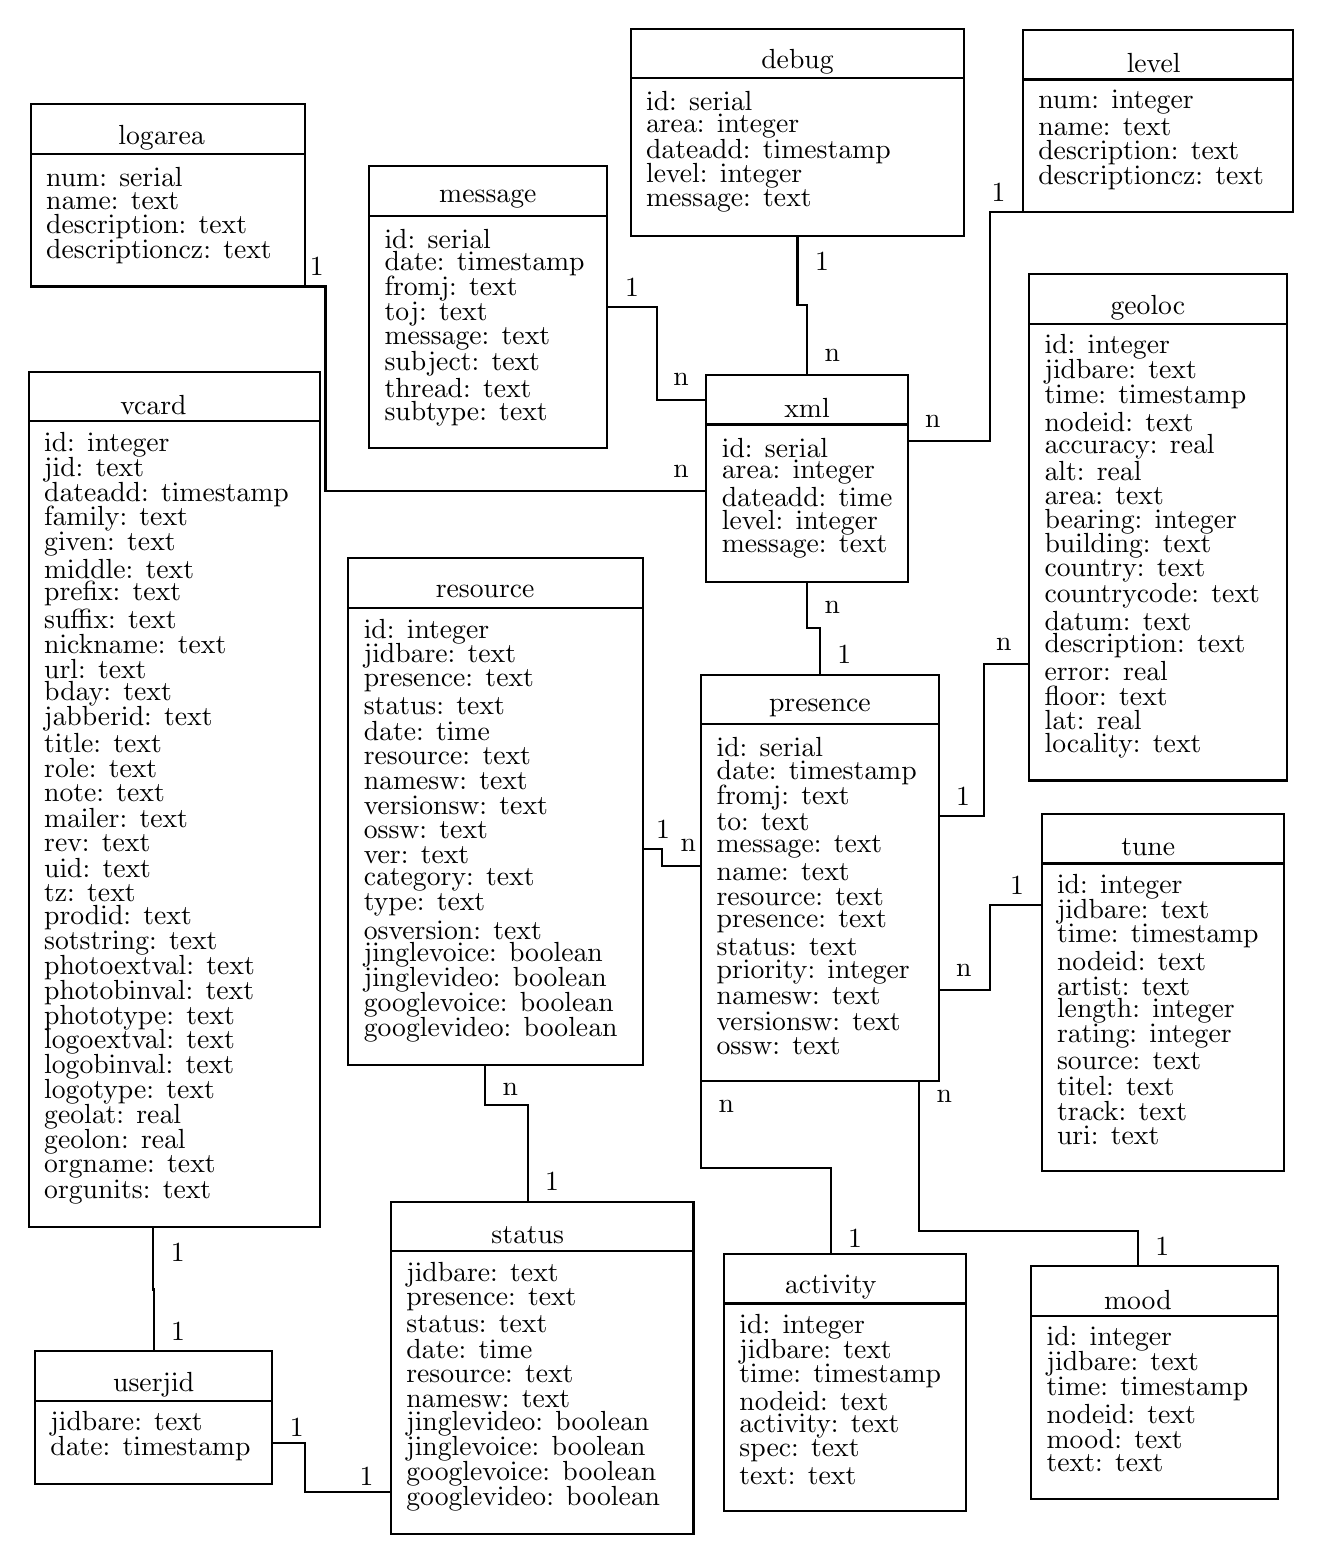
\begin{tikzpicture}
\pgftransformxscale{1.000000}
\pgftransformyscale{-1.000000}
\definecolor{dialinecolor}{rgb}{0.000000, 0.000000, 0.000000}
\pgfsetstrokecolor{dialinecolor}
\definecolor{dialinecolor}{rgb}{1.000000, 1.000000, 1.000000}
\pgfsetfillcolor{dialinecolor}
\pgfsetlinewidth{0.050000\du}
\pgfsetdash{}{0pt}
\definecolor{dialinecolor}{rgb}{1.000000, 1.000000, 1.000000}
\pgfsetfillcolor{dialinecolor}
\fill (-12.181150\du,-149.781000\du)--(-12.181150\du,-148.581000\du)--(-4.141150\du,-148.581000\du)--(-4.141150\du,-149.781000\du)--cycle;
\definecolor{dialinecolor}{rgb}{0.000000, 0.000000, 0.000000}
\pgfsetstrokecolor{dialinecolor}
\draw (-12.181150\du,-149.781000\du)--(-12.181150\du,-148.581000\du)--(-4.141150\du,-148.581000\du)--(-4.141150\du,-149.781000\du)--cycle;
% setfont left to latex
\definecolor{dialinecolor}{rgb}{0.000000, 0.000000, 0.000000}
\pgfsetstrokecolor{dialinecolor}
\node at (-8.161150\du,-148.981000\du){debug};
\definecolor{dialinecolor}{rgb}{1.000000, 1.000000, 1.000000}
\pgfsetfillcolor{dialinecolor}
\fill (-12.181150\du,-148.581000\du)--(-12.181150\du,-144.781000\du)--(-4.141150\du,-144.781000\du)--(-4.141150\du,-148.581000\du)--cycle;
\definecolor{dialinecolor}{rgb}{0.000000, 0.000000, 0.000000}
\pgfsetstrokecolor{dialinecolor}
\draw (-12.181150\du,-148.581000\du)--(-12.181150\du,-144.781000\du)--(-4.141150\du,-144.781000\du)--(-4.141150\du,-148.581000\du)--cycle;
% setfont left to latex
\definecolor{dialinecolor}{rgb}{0.000000, 0.000000, 0.000000}
\pgfsetstrokecolor{dialinecolor}
\node[anchor=west] at (-12.056150\du,-148.031000\du){ id: serial};
% setfont left to latex
\definecolor{dialinecolor}{rgb}{0.000000, 0.000000, 0.000000}
\pgfsetstrokecolor{dialinecolor}
\node[anchor=west] at (-12.056150\du,-147.431000\du){ area: integer};
% setfont left to latex
\definecolor{dialinecolor}{rgb}{0.000000, 0.000000, 0.000000}
\pgfsetstrokecolor{dialinecolor}
\node[anchor=west] at (-12.056150\du,-146.831000\du){ dateadd: timestamp};
% setfont left to latex
\definecolor{dialinecolor}{rgb}{0.000000, 0.000000, 0.000000}
\pgfsetstrokecolor{dialinecolor}
\node[anchor=west] at (-12.056150\du,-146.231000\du){ level: integer};
% setfont left to latex
\definecolor{dialinecolor}{rgb}{0.000000, 0.000000, 0.000000}
\pgfsetstrokecolor{dialinecolor}
\node[anchor=west] at (-12.056150\du,-145.631000\du){ message: text};
% setfont left to latex
\definecolor{dialinecolor}{rgb}{0.000000, 0.000000, 0.000000}
\pgfsetstrokecolor{dialinecolor}
\node[anchor=west] at (-12.056150\du,-145.031000\du){                          };
\pgfsetlinewidth{0.050000\du}
\pgfsetdash{}{0pt}
\definecolor{dialinecolor}{rgb}{1.000000, 1.000000, 1.000000}
\pgfsetfillcolor{dialinecolor}
\fill (-2.731200\du,-149.756000\du)--(-2.731200\du,-148.556000\du)--(3.768800\du,-148.556000\du)--(3.768800\du,-149.756000\du)--cycle;
\definecolor{dialinecolor}{rgb}{0.000000, 0.000000, 0.000000}
\pgfsetstrokecolor{dialinecolor}
\draw (-2.731200\du,-149.756000\du)--(-2.731200\du,-148.556000\du)--(3.768800\du,-148.556000\du)--(3.768800\du,-149.756000\du)--cycle;
% setfont left to latex
\definecolor{dialinecolor}{rgb}{0.000000, 0.000000, 0.000000}
\pgfsetstrokecolor{dialinecolor}
\node at (0.418800\du,-148.956000\du){level};
\definecolor{dialinecolor}{rgb}{1.000000, 1.000000, 1.000000}
\pgfsetfillcolor{dialinecolor}
\fill (-2.731200\du,-148.556000\du)--(-2.731200\du,-145.356000\du)--(3.768800\du,-145.356000\du)--(3.768800\du,-148.556000\du)--cycle;
\definecolor{dialinecolor}{rgb}{0.000000, 0.000000, 0.000000}
\pgfsetstrokecolor{dialinecolor}
\draw (-2.731200\du,-148.556000\du)--(-2.731200\du,-145.356000\du)--(3.768800\du,-145.356000\du)--(3.768800\du,-148.556000\du)--cycle;
% setfont left to latex
\definecolor{dialinecolor}{rgb}{0.000000, 0.000000, 0.000000}
\pgfsetstrokecolor{dialinecolor}
\node[anchor=west] at (-2.606200\du,-148.006000\du){ num: integer};
% setfont left to latex
\definecolor{dialinecolor}{rgb}{0.000000, 0.000000, 0.000000}
\pgfsetstrokecolor{dialinecolor}
\node[anchor=west] at (-2.606200\du,-147.406000\du){ name: text};
% setfont left to latex
\definecolor{dialinecolor}{rgb}{0.000000, 0.000000, 0.000000}
\pgfsetstrokecolor{dialinecolor}
\node[anchor=west] at (-2.606200\du,-146.806000\du){ description: text};
% setfont left to latex
\definecolor{dialinecolor}{rgb}{0.000000, 0.000000, 0.000000}
\pgfsetstrokecolor{dialinecolor}
\node[anchor=west] at (-2.606200\du,-146.206000\du){ descriptioncz: text};
% setfont left to latex
\definecolor{dialinecolor}{rgb}{0.000000, 0.000000, 0.000000}
\pgfsetstrokecolor{dialinecolor}
\node[anchor=west] at (-2.606200\du,-145.606000\du){ };
\pgfsetlinewidth{0.050000\du}
\pgfsetdash{}{0pt}
\definecolor{dialinecolor}{rgb}{1.000000, 1.000000, 1.000000}
\pgfsetfillcolor{dialinecolor}
\fill (-26.631050\du,-147.969000\du)--(-26.631050\du,-146.769000\du)--(-20.031050\du,-146.769000\du)--(-20.031050\du,-147.969000\du)--cycle;
\definecolor{dialinecolor}{rgb}{0.000000, 0.000000, 0.000000}
\pgfsetstrokecolor{dialinecolor}
\draw (-26.631050\du,-147.969000\du)--(-26.631050\du,-146.769000\du)--(-20.031050\du,-146.769000\du)--(-20.031050\du,-147.969000\du)--cycle;
% setfont left to latex
\definecolor{dialinecolor}{rgb}{0.000000, 0.000000, 0.000000}
\pgfsetstrokecolor{dialinecolor}
\node at (-23.481050\du,-147.169000\du){logarea};
\definecolor{dialinecolor}{rgb}{1.000000, 1.000000, 1.000000}
\pgfsetfillcolor{dialinecolor}
\fill (-26.631050\du,-146.769000\du)--(-26.631050\du,-143.569000\du)--(-20.031050\du,-143.569000\du)--(-20.031050\du,-146.769000\du)--cycle;
\definecolor{dialinecolor}{rgb}{0.000000, 0.000000, 0.000000}
\pgfsetstrokecolor{dialinecolor}
\draw (-26.631050\du,-146.769000\du)--(-26.631050\du,-143.569000\du)--(-20.031050\du,-143.569000\du)--(-20.031050\du,-146.769000\du)--cycle;
% setfont left to latex
\definecolor{dialinecolor}{rgb}{0.000000, 0.000000, 0.000000}
\pgfsetstrokecolor{dialinecolor}
\node[anchor=west] at (-26.506050\du,-146.219000\du){ num: serial};
% setfont left to latex
\definecolor{dialinecolor}{rgb}{0.000000, 0.000000, 0.000000}
\pgfsetstrokecolor{dialinecolor}
\node[anchor=west] at (-26.506050\du,-145.619000\du){ name: text};
% setfont left to latex
\definecolor{dialinecolor}{rgb}{0.000000, 0.000000, 0.000000}
\pgfsetstrokecolor{dialinecolor}
\node[anchor=west] at (-26.506050\du,-145.019000\du){ description: text};
% setfont left to latex
\definecolor{dialinecolor}{rgb}{0.000000, 0.000000, 0.000000}
\pgfsetstrokecolor{dialinecolor}
\node[anchor=west] at (-26.506050\du,-144.419000\du){ descriptioncz: text};
% setfont left to latex
\definecolor{dialinecolor}{rgb}{0.000000, 0.000000, 0.000000}
\pgfsetstrokecolor{dialinecolor}
\node[anchor=west] at (-26.506050\du,-143.819000\du){ };
\pgfsetlinewidth{0.050000\du}
\pgfsetdash{}{0pt}
\definecolor{dialinecolor}{rgb}{1.000000, 1.000000, 1.000000}
\pgfsetfillcolor{dialinecolor}
\fill (-18.481050\du,-146.469000\du)--(-18.481050\du,-145.269000\du)--(-12.761050\du,-145.269000\du)--(-12.761050\du,-146.469000\du)--cycle;
\definecolor{dialinecolor}{rgb}{0.000000, 0.000000, 0.000000}
\pgfsetstrokecolor{dialinecolor}
\draw (-18.481050\du,-146.469000\du)--(-18.481050\du,-145.269000\du)--(-12.761050\du,-145.269000\du)--(-12.761050\du,-146.469000\du)--cycle;
% setfont left to latex
\definecolor{dialinecolor}{rgb}{0.000000, 0.000000, 0.000000}
\pgfsetstrokecolor{dialinecolor}
\node at (-15.621050\du,-145.669000\du){message};
\definecolor{dialinecolor}{rgb}{1.000000, 1.000000, 1.000000}
\pgfsetfillcolor{dialinecolor}
\fill (-18.481050\du,-145.269000\du)--(-18.481050\du,-139.669000\du)--(-12.761050\du,-139.669000\du)--(-12.761050\du,-145.269000\du)--cycle;
\definecolor{dialinecolor}{rgb}{0.000000, 0.000000, 0.000000}
\pgfsetstrokecolor{dialinecolor}
\draw (-18.481050\du,-145.269000\du)--(-18.481050\du,-139.669000\du)--(-12.761050\du,-139.669000\du)--(-12.761050\du,-145.269000\du)--cycle;
% setfont left to latex
\definecolor{dialinecolor}{rgb}{0.000000, 0.000000, 0.000000}
\pgfsetstrokecolor{dialinecolor}
\node[anchor=west] at (-18.356050\du,-144.719000\du){ id: serial};
% setfont left to latex
\definecolor{dialinecolor}{rgb}{0.000000, 0.000000, 0.000000}
\pgfsetstrokecolor{dialinecolor}
\node[anchor=west] at (-18.356050\du,-144.119000\du){ date: timestamp};
% setfont left to latex
\definecolor{dialinecolor}{rgb}{0.000000, 0.000000, 0.000000}
\pgfsetstrokecolor{dialinecolor}
\node[anchor=west] at (-18.356050\du,-143.519000\du){ fromj: text};
% setfont left to latex
\definecolor{dialinecolor}{rgb}{0.000000, 0.000000, 0.000000}
\pgfsetstrokecolor{dialinecolor}
\node[anchor=west] at (-18.356050\du,-142.919000\du){ toj: text};
% setfont left to latex
\definecolor{dialinecolor}{rgb}{0.000000, 0.000000, 0.000000}
\pgfsetstrokecolor{dialinecolor}
\node[anchor=west] at (-18.356050\du,-142.319000\du){ message: text};
% setfont left to latex
\definecolor{dialinecolor}{rgb}{0.000000, 0.000000, 0.000000}
\pgfsetstrokecolor{dialinecolor}
\node[anchor=west] at (-18.356050\du,-141.719000\du){ subject: text};
% setfont left to latex
\definecolor{dialinecolor}{rgb}{0.000000, 0.000000, 0.000000}
\pgfsetstrokecolor{dialinecolor}
\node[anchor=west] at (-18.356050\du,-141.119000\du){ thread: text};
% setfont left to latex
\definecolor{dialinecolor}{rgb}{0.000000, 0.000000, 0.000000}
\pgfsetstrokecolor{dialinecolor}
\node[anchor=west] at (-18.356050\du,-140.519000\du){ subtype: text};
% setfont left to latex
\definecolor{dialinecolor}{rgb}{0.000000, 0.000000, 0.000000}
\pgfsetstrokecolor{dialinecolor}
\node[anchor=west] at (-18.356050\du,-139.919000\du){                  };
\pgfsetlinewidth{0.050000\du}
\pgfsetdash{}{0pt}
\definecolor{dialinecolor}{rgb}{1.000000, 1.000000, 1.000000}
\pgfsetfillcolor{dialinecolor}
\fill (-10.481100\du,-134.219000\du)--(-10.481100\du,-133.019000\du)--(-4.761100\du,-133.019000\du)--(-4.761100\du,-134.219000\du)--cycle;
\definecolor{dialinecolor}{rgb}{0.000000, 0.000000, 0.000000}
\pgfsetstrokecolor{dialinecolor}
\draw (-10.481100\du,-134.219000\du)--(-10.481100\du,-133.019000\du)--(-4.761100\du,-133.019000\du)--(-4.761100\du,-134.219000\du)--cycle;
% setfont left to latex
\definecolor{dialinecolor}{rgb}{0.000000, 0.000000, 0.000000}
\pgfsetstrokecolor{dialinecolor}
\node at (-7.621100\du,-133.419000\du){presence};
\definecolor{dialinecolor}{rgb}{1.000000, 1.000000, 1.000000}
\pgfsetfillcolor{dialinecolor}
\fill (-10.481100\du,-133.019000\du)--(-10.481100\du,-124.419000\du)--(-4.761100\du,-124.419000\du)--(-4.761100\du,-133.019000\du)--cycle;
\definecolor{dialinecolor}{rgb}{0.000000, 0.000000, 0.000000}
\pgfsetstrokecolor{dialinecolor}
\draw (-10.481100\du,-133.019000\du)--(-10.481100\du,-124.419000\du)--(-4.761100\du,-124.419000\du)--(-4.761100\du,-133.019000\du)--cycle;
% setfont left to latex
\definecolor{dialinecolor}{rgb}{0.000000, 0.000000, 0.000000}
\pgfsetstrokecolor{dialinecolor}
\node[anchor=west] at (-10.356100\du,-132.469000\du){ id: serial};
% setfont left to latex
\definecolor{dialinecolor}{rgb}{0.000000, 0.000000, 0.000000}
\pgfsetstrokecolor{dialinecolor}
\node[anchor=west] at (-10.356100\du,-131.869000\du){ date: timestamp};
% setfont left to latex
\definecolor{dialinecolor}{rgb}{0.000000, 0.000000, 0.000000}
\pgfsetstrokecolor{dialinecolor}
\node[anchor=west] at (-10.356100\du,-131.269000\du){ fromj: text};
% setfont left to latex
\definecolor{dialinecolor}{rgb}{0.000000, 0.000000, 0.000000}
\pgfsetstrokecolor{dialinecolor}
\node[anchor=west] at (-10.356100\du,-130.669000\du){ to: text};
% setfont left to latex
\definecolor{dialinecolor}{rgb}{0.000000, 0.000000, 0.000000}
\pgfsetstrokecolor{dialinecolor}
\node[anchor=west] at (-10.356100\du,-130.069000\du){ message: text};
% setfont left to latex
\definecolor{dialinecolor}{rgb}{0.000000, 0.000000, 0.000000}
\pgfsetstrokecolor{dialinecolor}
\node[anchor=west] at (-10.356100\du,-129.469000\du){ name: text};
% setfont left to latex
\definecolor{dialinecolor}{rgb}{0.000000, 0.000000, 0.000000}
\pgfsetstrokecolor{dialinecolor}
\node[anchor=west] at (-10.356100\du,-128.869000\du){ resource: text};
% setfont left to latex
\definecolor{dialinecolor}{rgb}{0.000000, 0.000000, 0.000000}
\pgfsetstrokecolor{dialinecolor}
\node[anchor=west] at (-10.356100\du,-128.269000\du){ presence: text};
% setfont left to latex
\definecolor{dialinecolor}{rgb}{0.000000, 0.000000, 0.000000}
\pgfsetstrokecolor{dialinecolor}
\node[anchor=west] at (-10.356100\du,-127.669000\du){ status: text};
% setfont left to latex
\definecolor{dialinecolor}{rgb}{0.000000, 0.000000, 0.000000}
\pgfsetstrokecolor{dialinecolor}
\node[anchor=west] at (-10.356100\du,-127.069000\du){ priority: integer};
% setfont left to latex
\definecolor{dialinecolor}{rgb}{0.000000, 0.000000, 0.000000}
\pgfsetstrokecolor{dialinecolor}
\node[anchor=west] at (-10.356100\du,-126.469000\du){ namesw: text};
% setfont left to latex
\definecolor{dialinecolor}{rgb}{0.000000, 0.000000, 0.000000}
\pgfsetstrokecolor{dialinecolor}
\node[anchor=west] at (-10.356100\du,-125.869000\du){ versionsw: text};
% setfont left to latex
\definecolor{dialinecolor}{rgb}{0.000000, 0.000000, 0.000000}
\pgfsetstrokecolor{dialinecolor}
\node[anchor=west] at (-10.356100\du,-125.269000\du){ ossw: text};
% setfont left to latex
\definecolor{dialinecolor}{rgb}{0.000000, 0.000000, 0.000000}
\pgfsetstrokecolor{dialinecolor}
\node[anchor=west] at (-10.356100\du,-124.669000\du){ };
\pgfsetlinewidth{0.050000\du}
\pgfsetdash{}{0pt}
\definecolor{dialinecolor}{rgb}{1.000000, 1.000000, 1.000000}
\pgfsetfillcolor{dialinecolor}
\fill (-26.531050\du,-117.919000\du)--(-26.531050\du,-116.719000\du)--(-20.811050\du,-116.719000\du)--(-20.811050\du,-117.919000\du)--cycle;
\definecolor{dialinecolor}{rgb}{0.000000, 0.000000, 0.000000}
\pgfsetstrokecolor{dialinecolor}
\draw (-26.531050\du,-117.919000\du)--(-26.531050\du,-116.719000\du)--(-20.811050\du,-116.719000\du)--(-20.811050\du,-117.919000\du)--cycle;
% setfont left to latex
\definecolor{dialinecolor}{rgb}{0.000000, 0.000000, 0.000000}
\pgfsetstrokecolor{dialinecolor}
\node at (-23.671050\du,-117.119000\du){userjid};
\definecolor{dialinecolor}{rgb}{1.000000, 1.000000, 1.000000}
\pgfsetfillcolor{dialinecolor}
\fill (-26.531050\du,-116.719000\du)--(-26.531050\du,-114.719000\du)--(-20.811050\du,-114.719000\du)--(-20.811050\du,-116.719000\du)--cycle;
\definecolor{dialinecolor}{rgb}{0.000000, 0.000000, 0.000000}
\pgfsetstrokecolor{dialinecolor}
\draw (-26.531050\du,-116.719000\du)--(-26.531050\du,-114.719000\du)--(-20.811050\du,-114.719000\du)--(-20.811050\du,-116.719000\du)--cycle;
% setfont left to latex
\definecolor{dialinecolor}{rgb}{0.000000, 0.000000, 0.000000}
\pgfsetstrokecolor{dialinecolor}
\node[anchor=west] at (-26.406050\du,-116.169000\du){ jidbare: text};
% setfont left to latex
\definecolor{dialinecolor}{rgb}{0.000000, 0.000000, 0.000000}
\pgfsetstrokecolor{dialinecolor}
\node[anchor=west] at (-26.406050\du,-115.569000\du){ date: timestamp};
% setfont left to latex
\definecolor{dialinecolor}{rgb}{0.000000, 0.000000, 0.000000}
\pgfsetstrokecolor{dialinecolor}
\node[anchor=west] at (-26.406050\du,-114.969000\du){                  };
\pgfsetlinewidth{0.050000\du}
\pgfsetdash{}{0pt}
\definecolor{dialinecolor}{rgb}{1.000000, 1.000000, 1.000000}
\pgfsetfillcolor{dialinecolor}
\fill (-26.681100\du,-141.519000\du)--(-26.681100\du,-140.319000\du)--(-19.671100\du,-140.319000\du)--(-19.671100\du,-141.519000\du)--cycle;
\definecolor{dialinecolor}{rgb}{0.000000, 0.000000, 0.000000}
\pgfsetstrokecolor{dialinecolor}
\draw (-26.681100\du,-141.519000\du)--(-26.681100\du,-140.319000\du)--(-19.671100\du,-140.319000\du)--(-19.671100\du,-141.519000\du)--cycle;
% setfont left to latex
\definecolor{dialinecolor}{rgb}{0.000000, 0.000000, 0.000000}
\pgfsetstrokecolor{dialinecolor}
\node at (-23.676100\du,-140.719000\du){vcard};
\definecolor{dialinecolor}{rgb}{1.000000, 1.000000, 1.000000}
\pgfsetfillcolor{dialinecolor}
\fill (-26.681100\du,-140.319000\du)--(-26.681100\du,-120.919000\du)--(-19.671100\du,-120.919000\du)--(-19.671100\du,-140.319000\du)--cycle;
\definecolor{dialinecolor}{rgb}{0.000000, 0.000000, 0.000000}
\pgfsetstrokecolor{dialinecolor}
\draw (-26.681100\du,-140.319000\du)--(-26.681100\du,-120.919000\du)--(-19.671100\du,-120.919000\du)--(-19.671100\du,-140.319000\du)--cycle;
% setfont left to latex
\definecolor{dialinecolor}{rgb}{0.000000, 0.000000, 0.000000}
\pgfsetstrokecolor{dialinecolor}
\node[anchor=west] at (-26.556100\du,-139.769000\du){ id: integer};
% setfont left to latex
\definecolor{dialinecolor}{rgb}{0.000000, 0.000000, 0.000000}
\pgfsetstrokecolor{dialinecolor}
\node[anchor=west] at (-26.556100\du,-139.169000\du){ jid: text};
% setfont left to latex
\definecolor{dialinecolor}{rgb}{0.000000, 0.000000, 0.000000}
\pgfsetstrokecolor{dialinecolor}
\node[anchor=west] at (-26.556100\du,-138.569000\du){ dateadd: timestamp};
% setfont left to latex
\definecolor{dialinecolor}{rgb}{0.000000, 0.000000, 0.000000}
\pgfsetstrokecolor{dialinecolor}
\node[anchor=west] at (-26.556100\du,-137.969000\du){ family: text};
% setfont left to latex
\definecolor{dialinecolor}{rgb}{0.000000, 0.000000, 0.000000}
\pgfsetstrokecolor{dialinecolor}
\node[anchor=west] at (-26.556100\du,-137.369000\du){ given: text};
% setfont left to latex
\definecolor{dialinecolor}{rgb}{0.000000, 0.000000, 0.000000}
\pgfsetstrokecolor{dialinecolor}
\node[anchor=west] at (-26.556100\du,-136.769000\du){ middle: text};
% setfont left to latex
\definecolor{dialinecolor}{rgb}{0.000000, 0.000000, 0.000000}
\pgfsetstrokecolor{dialinecolor}
\node[anchor=west] at (-26.556100\du,-136.169000\du){ prefix: text};
% setfont left to latex
\definecolor{dialinecolor}{rgb}{0.000000, 0.000000, 0.000000}
\pgfsetstrokecolor{dialinecolor}
\node[anchor=west] at (-26.556100\du,-135.569000\du){ suffix: text};
% setfont left to latex
\definecolor{dialinecolor}{rgb}{0.000000, 0.000000, 0.000000}
\pgfsetstrokecolor{dialinecolor}
\node[anchor=west] at (-26.556100\du,-134.969000\du){ nickname: text};
% setfont left to latex
\definecolor{dialinecolor}{rgb}{0.000000, 0.000000, 0.000000}
\pgfsetstrokecolor{dialinecolor}
\node[anchor=west] at (-26.556100\du,-134.369000\du){ url: text};
% setfont left to latex
\definecolor{dialinecolor}{rgb}{0.000000, 0.000000, 0.000000}
\pgfsetstrokecolor{dialinecolor}
\node[anchor=west] at (-26.556100\du,-133.769000\du){ bday: text};
% setfont left to latex
\definecolor{dialinecolor}{rgb}{0.000000, 0.000000, 0.000000}
\pgfsetstrokecolor{dialinecolor}
\node[anchor=west] at (-26.556100\du,-133.169000\du){ jabberid: text};
% setfont left to latex
\definecolor{dialinecolor}{rgb}{0.000000, 0.000000, 0.000000}
\pgfsetstrokecolor{dialinecolor}
\node[anchor=west] at (-26.556100\du,-132.569000\du){ title: text};
% setfont left to latex
\definecolor{dialinecolor}{rgb}{0.000000, 0.000000, 0.000000}
\pgfsetstrokecolor{dialinecolor}
\node[anchor=west] at (-26.556100\du,-131.969000\du){ role: text};
% setfont left to latex
\definecolor{dialinecolor}{rgb}{0.000000, 0.000000, 0.000000}
\pgfsetstrokecolor{dialinecolor}
\node[anchor=west] at (-26.556100\du,-131.369000\du){ note: text};
% setfont left to latex
\definecolor{dialinecolor}{rgb}{0.000000, 0.000000, 0.000000}
\pgfsetstrokecolor{dialinecolor}
\node[anchor=west] at (-26.556100\du,-130.769000\du){ mailer: text};
% setfont left to latex
\definecolor{dialinecolor}{rgb}{0.000000, 0.000000, 0.000000}
\pgfsetstrokecolor{dialinecolor}
\node[anchor=west] at (-26.556100\du,-130.169000\du){ rev: text};
% setfont left to latex
\definecolor{dialinecolor}{rgb}{0.000000, 0.000000, 0.000000}
\pgfsetstrokecolor{dialinecolor}
\node[anchor=west] at (-26.556100\du,-129.569000\du){ uid: text};
% setfont left to latex
\definecolor{dialinecolor}{rgb}{0.000000, 0.000000, 0.000000}
\pgfsetstrokecolor{dialinecolor}
\node[anchor=west] at (-26.556100\du,-128.969000\du){ tz: text};
% setfont left to latex
\definecolor{dialinecolor}{rgb}{0.000000, 0.000000, 0.000000}
\pgfsetstrokecolor{dialinecolor}
\node[anchor=west] at (-26.556100\du,-128.369000\du){ prodid: text};
% setfont left to latex
\definecolor{dialinecolor}{rgb}{0.000000, 0.000000, 0.000000}
\pgfsetstrokecolor{dialinecolor}
\node[anchor=west] at (-26.556100\du,-127.769000\du){ sotstring: text};
% setfont left to latex
\definecolor{dialinecolor}{rgb}{0.000000, 0.000000, 0.000000}
\pgfsetstrokecolor{dialinecolor}
\node[anchor=west] at (-26.556100\du,-127.169000\du){ photoextval: text};
% setfont left to latex
\definecolor{dialinecolor}{rgb}{0.000000, 0.000000, 0.000000}
\pgfsetstrokecolor{dialinecolor}
\node[anchor=west] at (-26.556100\du,-126.569000\du){ photobinval: text};
% setfont left to latex
\definecolor{dialinecolor}{rgb}{0.000000, 0.000000, 0.000000}
\pgfsetstrokecolor{dialinecolor}
\node[anchor=west] at (-26.556100\du,-125.969000\du){ phototype: text};
% setfont left to latex
\definecolor{dialinecolor}{rgb}{0.000000, 0.000000, 0.000000}
\pgfsetstrokecolor{dialinecolor}
\node[anchor=west] at (-26.556100\du,-125.369000\du){ logoextval: text};
% setfont left to latex
\definecolor{dialinecolor}{rgb}{0.000000, 0.000000, 0.000000}
\pgfsetstrokecolor{dialinecolor}
\node[anchor=west] at (-26.556100\du,-124.769000\du){ logobinval: text};
% setfont left to latex
\definecolor{dialinecolor}{rgb}{0.000000, 0.000000, 0.000000}
\pgfsetstrokecolor{dialinecolor}
\node[anchor=west] at (-26.556100\du,-124.169000\du){ logotype: text};
% setfont left to latex
\definecolor{dialinecolor}{rgb}{0.000000, 0.000000, 0.000000}
\pgfsetstrokecolor{dialinecolor}
\node[anchor=west] at (-26.556100\du,-123.569000\du){ geolat: real};
% setfont left to latex
\definecolor{dialinecolor}{rgb}{0.000000, 0.000000, 0.000000}
\pgfsetstrokecolor{dialinecolor}
\node[anchor=west] at (-26.556100\du,-122.969000\du){ geolon: real};
% setfont left to latex
\definecolor{dialinecolor}{rgb}{0.000000, 0.000000, 0.000000}
\pgfsetstrokecolor{dialinecolor}
\node[anchor=west] at (-26.556100\du,-122.369000\du){ orgname: text};
% setfont left to latex
\definecolor{dialinecolor}{rgb}{0.000000, 0.000000, 0.000000}
\pgfsetstrokecolor{dialinecolor}
\node[anchor=west] at (-26.556100\du,-121.769000\du){ orgunits: text};
% setfont left to latex
\definecolor{dialinecolor}{rgb}{0.000000, 0.000000, 0.000000}
\pgfsetstrokecolor{dialinecolor}
\node[anchor=west] at (-26.556100\du,-121.169000\du){ };
\pgfsetlinewidth{0.050000\du}
\pgfsetdash{}{0pt}
\definecolor{dialinecolor}{rgb}{1.000000, 1.000000, 1.000000}
\pgfsetfillcolor{dialinecolor}
\fill (-10.356000\du,-141.444000\du)--(-10.356000\du,-140.244000\du)--(-5.506000\du,-140.244000\du)--(-5.506000\du,-141.444000\du)--cycle;
\definecolor{dialinecolor}{rgb}{0.000000, 0.000000, 0.000000}
\pgfsetstrokecolor{dialinecolor}
\draw (-10.356000\du,-141.444000\du)--(-10.356000\du,-140.244000\du)--(-5.506000\du,-140.244000\du)--(-5.506000\du,-141.444000\du)--cycle;
% setfont left to latex
\definecolor{dialinecolor}{rgb}{0.000000, 0.000000, 0.000000}
\pgfsetstrokecolor{dialinecolor}
\node at (-7.931000\du,-140.644000\du){xml};
\definecolor{dialinecolor}{rgb}{1.000000, 1.000000, 1.000000}
\pgfsetfillcolor{dialinecolor}
\fill (-10.356000\du,-140.244000\du)--(-10.356000\du,-136.444000\du)--(-5.506000\du,-136.444000\du)--(-5.506000\du,-140.244000\du)--cycle;
\definecolor{dialinecolor}{rgb}{0.000000, 0.000000, 0.000000}
\pgfsetstrokecolor{dialinecolor}
\draw (-10.356000\du,-140.244000\du)--(-10.356000\du,-136.444000\du)--(-5.506000\du,-136.444000\du)--(-5.506000\du,-140.244000\du)--cycle;
% setfont left to latex
\definecolor{dialinecolor}{rgb}{0.000000, 0.000000, 0.000000}
\pgfsetstrokecolor{dialinecolor}
\node[anchor=west] at (-10.231000\du,-139.694000\du){ id: serial};
% setfont left to latex
\definecolor{dialinecolor}{rgb}{0.000000, 0.000000, 0.000000}
\pgfsetstrokecolor{dialinecolor}
\node[anchor=west] at (-10.231000\du,-139.094000\du){ area: integer};
% setfont left to latex
\definecolor{dialinecolor}{rgb}{0.000000, 0.000000, 0.000000}
\pgfsetstrokecolor{dialinecolor}
\node[anchor=west] at (-10.231000\du,-138.494000\du){ dateadd: time};
% setfont left to latex
\definecolor{dialinecolor}{rgb}{0.000000, 0.000000, 0.000000}
\pgfsetstrokecolor{dialinecolor}
\node[anchor=west] at (-10.231000\du,-137.894000\du){ level: integer};
% setfont left to latex
\definecolor{dialinecolor}{rgb}{0.000000, 0.000000, 0.000000}
\pgfsetstrokecolor{dialinecolor}
\node[anchor=west] at (-10.231000\du,-137.294000\du){ message: text};
% setfont left to latex
\definecolor{dialinecolor}{rgb}{0.000000, 0.000000, 0.000000}
\pgfsetstrokecolor{dialinecolor}
\node[anchor=west] at (-10.231000\du,-136.694000\du){ };
\pgfsetlinewidth{0.050000\du}
\pgfsetdash{}{0pt}
\definecolor{dialinecolor}{rgb}{1.000000, 1.000000, 1.000000}
\pgfsetfillcolor{dialinecolor}
\fill (-17.956050\du,-121.525000\du)--(-17.956050\du,-120.325000\du)--(-10.666050\du,-120.325000\du)--(-10.666050\du,-121.525000\du)--cycle;
\definecolor{dialinecolor}{rgb}{0.000000, 0.000000, 0.000000}
\pgfsetstrokecolor{dialinecolor}
\draw (-17.956050\du,-121.525000\du)--(-17.956050\du,-120.325000\du)--(-10.666050\du,-120.325000\du)--(-10.666050\du,-121.525000\du)--cycle;
% setfont left to latex
\definecolor{dialinecolor}{rgb}{0.000000, 0.000000, 0.000000}
\pgfsetstrokecolor{dialinecolor}
\node at (-14.661050\du,-120.725000\du){status};
\definecolor{dialinecolor}{rgb}{1.000000, 1.000000, 1.000000}
\pgfsetfillcolor{dialinecolor}
\fill (-17.956050\du,-120.325000\du)--(-17.956050\du,-113.525000\du)--(-10.666050\du,-113.525000\du)--(-10.666050\du,-120.325000\du)--cycle;
\definecolor{dialinecolor}{rgb}{0.000000, 0.000000, 0.000000}
\pgfsetstrokecolor{dialinecolor}
\draw (-17.956050\du,-120.325000\du)--(-17.956050\du,-113.525000\du)--(-10.666050\du,-113.525000\du)--(-10.666050\du,-120.325000\du)--cycle;
% setfont left to latex
\definecolor{dialinecolor}{rgb}{0.000000, 0.000000, 0.000000}
\pgfsetstrokecolor{dialinecolor}
\node[anchor=west] at (-17.831050\du,-119.775000\du){ jidbare: text};
% setfont left to latex
\definecolor{dialinecolor}{rgb}{0.000000, 0.000000, 0.000000}
\pgfsetstrokecolor{dialinecolor}
\node[anchor=west] at (-17.831050\du,-119.175000\du){ presence: text};
% setfont left to latex
\definecolor{dialinecolor}{rgb}{0.000000, 0.000000, 0.000000}
\pgfsetstrokecolor{dialinecolor}
\node[anchor=west] at (-17.831050\du,-118.575000\du){ status: text};
% setfont left to latex
\definecolor{dialinecolor}{rgb}{0.000000, 0.000000, 0.000000}
\pgfsetstrokecolor{dialinecolor}
\node[anchor=west] at (-17.831050\du,-117.975000\du){ date: time};
% setfont left to latex
\definecolor{dialinecolor}{rgb}{0.000000, 0.000000, 0.000000}
\pgfsetstrokecolor{dialinecolor}
\node[anchor=west] at (-17.831050\du,-117.375000\du){ resource: text};
% setfont left to latex
\definecolor{dialinecolor}{rgb}{0.000000, 0.000000, 0.000000}
\pgfsetstrokecolor{dialinecolor}
\node[anchor=west] at (-17.831050\du,-116.775000\du){ namesw: text};
% setfont left to latex
\definecolor{dialinecolor}{rgb}{0.000000, 0.000000, 0.000000}
\pgfsetstrokecolor{dialinecolor}
\node[anchor=west] at (-17.831050\du,-116.175000\du){ jinglevideo: boolean};
% setfont left to latex
\definecolor{dialinecolor}{rgb}{0.000000, 0.000000, 0.000000}
\pgfsetstrokecolor{dialinecolor}
\node[anchor=west] at (-17.831050\du,-115.575000\du){ jinglevoice: boolean};
% setfont left to latex
\definecolor{dialinecolor}{rgb}{0.000000, 0.000000, 0.000000}
\pgfsetstrokecolor{dialinecolor}
\node[anchor=west] at (-17.831050\du,-114.975000\du){ googlevoice: boolean};
% setfont left to latex
\definecolor{dialinecolor}{rgb}{0.000000, 0.000000, 0.000000}
\pgfsetstrokecolor{dialinecolor}
\node[anchor=west] at (-17.831050\du,-114.375000\du){ googlevideo: boolean};
% setfont left to latex
\definecolor{dialinecolor}{rgb}{0.000000, 0.000000, 0.000000}
\pgfsetstrokecolor{dialinecolor}
\node[anchor=west] at (-17.831050\du,-113.775000\du){ };
\pgfsetlinewidth{0.050000\du}
\pgfsetdash{}{0pt}
\definecolor{dialinecolor}{rgb}{1.000000, 1.000000, 1.000000}
\pgfsetfillcolor{dialinecolor}
\fill (-2.281100\du,-130.869375\du)--(-2.281100\du,-129.669375\du)--(3.558900\du,-129.669375\du)--(3.558900\du,-130.869375\du)--cycle;
\definecolor{dialinecolor}{rgb}{0.000000, 0.000000, 0.000000}
\pgfsetstrokecolor{dialinecolor}
\draw (-2.281100\du,-130.869375\du)--(-2.281100\du,-129.669375\du)--(3.558900\du,-129.669375\du)--(3.558900\du,-130.869375\du)--cycle;
% setfont left to latex
\definecolor{dialinecolor}{rgb}{0.000000, 0.000000, 0.000000}
\pgfsetstrokecolor{dialinecolor}
\node at (0.288900\du,-130.069375\du){tune};
\definecolor{dialinecolor}{rgb}{1.000000, 1.000000, 1.000000}
\pgfsetfillcolor{dialinecolor}
\fill (-2.281100\du,-129.669375\du)--(-2.281100\du,-122.269375\du)--(3.558900\du,-122.269375\du)--(3.558900\du,-129.669375\du)--cycle;
\definecolor{dialinecolor}{rgb}{0.000000, 0.000000, 0.000000}
\pgfsetstrokecolor{dialinecolor}
\draw (-2.281100\du,-129.669375\du)--(-2.281100\du,-122.269375\du)--(3.558900\du,-122.269375\du)--(3.558900\du,-129.669375\du)--cycle;
% setfont left to latex
\definecolor{dialinecolor}{rgb}{0.000000, 0.000000, 0.000000}
\pgfsetstrokecolor{dialinecolor}
\node[anchor=west] at (-2.156100\du,-129.119375\du){ id: integer};
% setfont left to latex
\definecolor{dialinecolor}{rgb}{0.000000, 0.000000, 0.000000}
\pgfsetstrokecolor{dialinecolor}
\node[anchor=west] at (-2.156100\du,-128.519375\du){ jidbare: text};
% setfont left to latex
\definecolor{dialinecolor}{rgb}{0.000000, 0.000000, 0.000000}
\pgfsetstrokecolor{dialinecolor}
\node[anchor=west] at (-2.156100\du,-127.919375\du){ time: timestamp};
% setfont left to latex
\definecolor{dialinecolor}{rgb}{0.000000, 0.000000, 0.000000}
\pgfsetstrokecolor{dialinecolor}
\node[anchor=west] at (-2.156100\du,-127.319375\du){ nodeid: text};
% setfont left to latex
\definecolor{dialinecolor}{rgb}{0.000000, 0.000000, 0.000000}
\pgfsetstrokecolor{dialinecolor}
\node[anchor=west] at (-2.156100\du,-126.719375\du){ artist: text};
% setfont left to latex
\definecolor{dialinecolor}{rgb}{0.000000, 0.000000, 0.000000}
\pgfsetstrokecolor{dialinecolor}
\node[anchor=west] at (-2.156100\du,-126.119375\du){ length: integer};
% setfont left to latex
\definecolor{dialinecolor}{rgb}{0.000000, 0.000000, 0.000000}
\pgfsetstrokecolor{dialinecolor}
\node[anchor=west] at (-2.156100\du,-125.519375\du){ rating: integer};
% setfont left to latex
\definecolor{dialinecolor}{rgb}{0.000000, 0.000000, 0.000000}
\pgfsetstrokecolor{dialinecolor}
\node[anchor=west] at (-2.156100\du,-124.919375\du){ source: text};
% setfont left to latex
\definecolor{dialinecolor}{rgb}{0.000000, 0.000000, 0.000000}
\pgfsetstrokecolor{dialinecolor}
\node[anchor=west] at (-2.156100\du,-124.319375\du){ titel: text};
% setfont left to latex
\definecolor{dialinecolor}{rgb}{0.000000, 0.000000, 0.000000}
\pgfsetstrokecolor{dialinecolor}
\node[anchor=west] at (-2.156100\du,-123.719375\du){ track: text};
% setfont left to latex
\definecolor{dialinecolor}{rgb}{0.000000, 0.000000, 0.000000}
\pgfsetstrokecolor{dialinecolor}
\node[anchor=west] at (-2.156100\du,-123.119375\du){ uri: text};
% setfont left to latex
\definecolor{dialinecolor}{rgb}{0.000000, 0.000000, 0.000000}
\pgfsetstrokecolor{dialinecolor}
\node[anchor=west] at (-2.156100\du,-122.519375\du){ };
\pgfsetlinewidth{0.050000\du}
\pgfsetdash{}{0pt}
\definecolor{dialinecolor}{rgb}{1.000000, 1.000000, 1.000000}
\pgfsetfillcolor{dialinecolor}
\fill (-2.581100\du,-143.869375\du)--(-2.581100\du,-142.669375\du)--(3.638900\du,-142.669375\du)--(3.638900\du,-143.869375\du)--cycle;
\definecolor{dialinecolor}{rgb}{0.000000, 0.000000, 0.000000}
\pgfsetstrokecolor{dialinecolor}
\draw (-2.581100\du,-143.869375\du)--(-2.581100\du,-142.669375\du)--(3.638900\du,-142.669375\du)--(3.638900\du,-143.869375\du)--cycle;
% setfont left to latex
\definecolor{dialinecolor}{rgb}{0.000000, 0.000000, 0.000000}
\pgfsetstrokecolor{dialinecolor}
\node at (0.278900\du,-143.069375\du){geoloc};
\definecolor{dialinecolor}{rgb}{1.000000, 1.000000, 1.000000}
\pgfsetfillcolor{dialinecolor}
\fill (-2.581100\du,-142.669375\du)--(-2.581100\du,-131.669375\du)--(3.638900\du,-131.669375\du)--(3.638900\du,-142.669375\du)--cycle;
\definecolor{dialinecolor}{rgb}{0.000000, 0.000000, 0.000000}
\pgfsetstrokecolor{dialinecolor}
\draw (-2.581100\du,-142.669375\du)--(-2.581100\du,-131.669375\du)--(3.638900\du,-131.669375\du)--(3.638900\du,-142.669375\du)--cycle;
% setfont left to latex
\definecolor{dialinecolor}{rgb}{0.000000, 0.000000, 0.000000}
\pgfsetstrokecolor{dialinecolor}
\node[anchor=west] at (-2.456100\du,-142.119375\du){ id: integer};
% setfont left to latex
\definecolor{dialinecolor}{rgb}{0.000000, 0.000000, 0.000000}
\pgfsetstrokecolor{dialinecolor}
\node[anchor=west] at (-2.456100\du,-141.519375\du){ jidbare: text};
% setfont left to latex
\definecolor{dialinecolor}{rgb}{0.000000, 0.000000, 0.000000}
\pgfsetstrokecolor{dialinecolor}
\node[anchor=west] at (-2.456100\du,-140.919375\du){ time: timestamp};
% setfont left to latex
\definecolor{dialinecolor}{rgb}{0.000000, 0.000000, 0.000000}
\pgfsetstrokecolor{dialinecolor}
\node[anchor=west] at (-2.456100\du,-140.319375\du){ nodeid: text};
% setfont left to latex
\definecolor{dialinecolor}{rgb}{0.000000, 0.000000, 0.000000}
\pgfsetstrokecolor{dialinecolor}
\node[anchor=west] at (-2.456100\du,-139.719375\du){ accuracy: real};
% setfont left to latex
\definecolor{dialinecolor}{rgb}{0.000000, 0.000000, 0.000000}
\pgfsetstrokecolor{dialinecolor}
\node[anchor=west] at (-2.456100\du,-139.119375\du){ alt: real};
% setfont left to latex
\definecolor{dialinecolor}{rgb}{0.000000, 0.000000, 0.000000}
\pgfsetstrokecolor{dialinecolor}
\node[anchor=west] at (-2.456100\du,-138.519375\du){ area: text};
% setfont left to latex
\definecolor{dialinecolor}{rgb}{0.000000, 0.000000, 0.000000}
\pgfsetstrokecolor{dialinecolor}
\node[anchor=west] at (-2.456100\du,-137.919375\du){ bearing: integer};
% setfont left to latex
\definecolor{dialinecolor}{rgb}{0.000000, 0.000000, 0.000000}
\pgfsetstrokecolor{dialinecolor}
\node[anchor=west] at (-2.456100\du,-137.319375\du){ building: text};
% setfont left to latex
\definecolor{dialinecolor}{rgb}{0.000000, 0.000000, 0.000000}
\pgfsetstrokecolor{dialinecolor}
\node[anchor=west] at (-2.456100\du,-136.719375\du){ country: text};
% setfont left to latex
\definecolor{dialinecolor}{rgb}{0.000000, 0.000000, 0.000000}
\pgfsetstrokecolor{dialinecolor}
\node[anchor=west] at (-2.456100\du,-136.119375\du){ countrycode: text};
% setfont left to latex
\definecolor{dialinecolor}{rgb}{0.000000, 0.000000, 0.000000}
\pgfsetstrokecolor{dialinecolor}
\node[anchor=west] at (-2.456100\du,-135.519375\du){ datum: text};
% setfont left to latex
\definecolor{dialinecolor}{rgb}{0.000000, 0.000000, 0.000000}
\pgfsetstrokecolor{dialinecolor}
\node[anchor=west] at (-2.456100\du,-134.919375\du){ description: text};
% setfont left to latex
\definecolor{dialinecolor}{rgb}{0.000000, 0.000000, 0.000000}
\pgfsetstrokecolor{dialinecolor}
\node[anchor=west] at (-2.456100\du,-134.319375\du){ error: real};
% setfont left to latex
\definecolor{dialinecolor}{rgb}{0.000000, 0.000000, 0.000000}
\pgfsetstrokecolor{dialinecolor}
\node[anchor=west] at (-2.456100\du,-133.719375\du){ floor: text};
% setfont left to latex
\definecolor{dialinecolor}{rgb}{0.000000, 0.000000, 0.000000}
\pgfsetstrokecolor{dialinecolor}
\node[anchor=west] at (-2.456100\du,-133.119375\du){ lat: real};
% setfont left to latex
\definecolor{dialinecolor}{rgb}{0.000000, 0.000000, 0.000000}
\pgfsetstrokecolor{dialinecolor}
\node[anchor=west] at (-2.456100\du,-132.519375\du){ locality: text};
% setfont left to latex
\definecolor{dialinecolor}{rgb}{0.000000, 0.000000, 0.000000}
\pgfsetstrokecolor{dialinecolor}
\node[anchor=west] at (-2.456100\du,-131.919375\du){ };
\pgfsetlinewidth{0.050000\du}
\pgfsetdash{}{0pt}
\definecolor{dialinecolor}{rgb}{1.000000, 1.000000, 1.000000}
\pgfsetfillcolor{dialinecolor}
\fill (-9.931100\du,-120.269375\du)--(-9.931100\du,-119.069375\du)--(-4.091100\du,-119.069375\du)--(-4.091100\du,-120.269375\du)--cycle;
\definecolor{dialinecolor}{rgb}{0.000000, 0.000000, 0.000000}
\pgfsetstrokecolor{dialinecolor}
\draw (-9.931100\du,-120.269375\du)--(-9.931100\du,-119.069375\du)--(-4.091100\du,-119.069375\du)--(-4.091100\du,-120.269375\du)--cycle;
% setfont left to latex
\definecolor{dialinecolor}{rgb}{0.000000, 0.000000, 0.000000}
\pgfsetstrokecolor{dialinecolor}
\node at (-7.361100\du,-119.469375\du){activity};
\definecolor{dialinecolor}{rgb}{1.000000, 1.000000, 1.000000}
\pgfsetfillcolor{dialinecolor}
\fill (-9.931100\du,-119.069375\du)--(-9.931100\du,-114.069375\du)--(-4.091100\du,-114.069375\du)--(-4.091100\du,-119.069375\du)--cycle;
\definecolor{dialinecolor}{rgb}{0.000000, 0.000000, 0.000000}
\pgfsetstrokecolor{dialinecolor}
\draw (-9.931100\du,-119.069375\du)--(-9.931100\du,-114.069375\du)--(-4.091100\du,-114.069375\du)--(-4.091100\du,-119.069375\du)--cycle;
% setfont left to latex
\definecolor{dialinecolor}{rgb}{0.000000, 0.000000, 0.000000}
\pgfsetstrokecolor{dialinecolor}
\node[anchor=west] at (-9.806100\du,-118.519375\du){ id: integer};
% setfont left to latex
\definecolor{dialinecolor}{rgb}{0.000000, 0.000000, 0.000000}
\pgfsetstrokecolor{dialinecolor}
\node[anchor=west] at (-9.806100\du,-117.919375\du){ jidbare: text};
% setfont left to latex
\definecolor{dialinecolor}{rgb}{0.000000, 0.000000, 0.000000}
\pgfsetstrokecolor{dialinecolor}
\node[anchor=west] at (-9.806100\du,-117.319375\du){ time: timestamp};
% setfont left to latex
\definecolor{dialinecolor}{rgb}{0.000000, 0.000000, 0.000000}
\pgfsetstrokecolor{dialinecolor}
\node[anchor=west] at (-9.806100\du,-116.719375\du){ nodeid: text};
% setfont left to latex
\definecolor{dialinecolor}{rgb}{0.000000, 0.000000, 0.000000}
\pgfsetstrokecolor{dialinecolor}
\node[anchor=west] at (-9.806100\du,-116.119375\du){ activity: text};
% setfont left to latex
\definecolor{dialinecolor}{rgb}{0.000000, 0.000000, 0.000000}
\pgfsetstrokecolor{dialinecolor}
\node[anchor=west] at (-9.806100\du,-115.519375\du){ spec: text};
% setfont left to latex
\definecolor{dialinecolor}{rgb}{0.000000, 0.000000, 0.000000}
\pgfsetstrokecolor{dialinecolor}
\node[anchor=west] at (-9.806100\du,-114.919375\du){ text: text};
% setfont left to latex
\definecolor{dialinecolor}{rgb}{0.000000, 0.000000, 0.000000}
\pgfsetstrokecolor{dialinecolor}
\node[anchor=west] at (-9.806100\du,-114.319375\du){ };
\pgfsetlinewidth{0.050000\du}
\pgfsetdash{}{0pt}
\definecolor{dialinecolor}{rgb}{1.000000, 1.000000, 1.000000}
\pgfsetfillcolor{dialinecolor}
\fill (-2.531100\du,-119.969375\du)--(-2.531100\du,-118.769375\du)--(3.408900\du,-118.769375\du)--(3.408900\du,-119.969375\du)--cycle;
\definecolor{dialinecolor}{rgb}{0.000000, 0.000000, 0.000000}
\pgfsetstrokecolor{dialinecolor}
\draw (-2.531100\du,-119.969375\du)--(-2.531100\du,-118.769375\du)--(3.408900\du,-118.769375\du)--(3.408900\du,-119.969375\du)--cycle;
% setfont left to latex
\definecolor{dialinecolor}{rgb}{0.000000, 0.000000, 0.000000}
\pgfsetstrokecolor{dialinecolor}
\node at (0.038900\du,-119.169375\du){mood};
\definecolor{dialinecolor}{rgb}{1.000000, 1.000000, 1.000000}
\pgfsetfillcolor{dialinecolor}
\fill (-2.531100\du,-118.769375\du)--(-2.531100\du,-114.369375\du)--(3.408900\du,-114.369375\du)--(3.408900\du,-118.769375\du)--cycle;
\definecolor{dialinecolor}{rgb}{0.000000, 0.000000, 0.000000}
\pgfsetstrokecolor{dialinecolor}
\draw (-2.531100\du,-118.769375\du)--(-2.531100\du,-114.369375\du)--(3.408900\du,-114.369375\du)--(3.408900\du,-118.769375\du)--cycle;
% setfont left to latex
\definecolor{dialinecolor}{rgb}{0.000000, 0.000000, 0.000000}
\pgfsetstrokecolor{dialinecolor}
\node[anchor=west] at (-2.406100\du,-118.219375\du){ id: integer};
% setfont left to latex
\definecolor{dialinecolor}{rgb}{0.000000, 0.000000, 0.000000}
\pgfsetstrokecolor{dialinecolor}
\node[anchor=west] at (-2.406100\du,-117.619375\du){ jidbare: text};
% setfont left to latex
\definecolor{dialinecolor}{rgb}{0.000000, 0.000000, 0.000000}
\pgfsetstrokecolor{dialinecolor}
\node[anchor=west] at (-2.406100\du,-117.019375\du){ time: timestamp};
% setfont left to latex
\definecolor{dialinecolor}{rgb}{0.000000, 0.000000, 0.000000}
\pgfsetstrokecolor{dialinecolor}
\node[anchor=west] at (-2.406100\du,-116.419375\du){ nodeid: text};
% setfont left to latex
\definecolor{dialinecolor}{rgb}{0.000000, 0.000000, 0.000000}
\pgfsetstrokecolor{dialinecolor}
\node[anchor=west] at (-2.406100\du,-115.819375\du){ mood: text};
% setfont left to latex
\definecolor{dialinecolor}{rgb}{0.000000, 0.000000, 0.000000}
\pgfsetstrokecolor{dialinecolor}
\node[anchor=west] at (-2.406100\du,-115.219375\du){ text: text};
% setfont left to latex
\definecolor{dialinecolor}{rgb}{0.000000, 0.000000, 0.000000}
\pgfsetstrokecolor{dialinecolor}
\node[anchor=west] at (-2.406100\du,-114.619375\du){ };
\pgfsetlinewidth{0.050000\du}
\pgfsetdash{}{0pt}
\definecolor{dialinecolor}{rgb}{1.000000, 1.000000, 1.000000}
\pgfsetfillcolor{dialinecolor}
\fill (-18.981100\du,-137.019375\du)--(-18.981100\du,-135.819375\du)--(-11.891100\du,-135.819375\du)--(-11.891100\du,-137.019375\du)--cycle;
\definecolor{dialinecolor}{rgb}{0.000000, 0.000000, 0.000000}
\pgfsetstrokecolor{dialinecolor}
\draw (-18.981100\du,-137.019375\du)--(-18.981100\du,-135.819375\du)--(-11.891100\du,-135.819375\du)--(-11.891100\du,-137.019375\du)--cycle;
% setfont left to latex
\definecolor{dialinecolor}{rgb}{0.000000, 0.000000, 0.000000}
\pgfsetstrokecolor{dialinecolor}
\node at (-15.686100\du,-136.219375\du){resource};
\definecolor{dialinecolor}{rgb}{1.000000, 1.000000, 1.000000}
\pgfsetfillcolor{dialinecolor}
\fill (-18.981100\du,-135.819375\du)--(-18.981100\du,-124.819375\du)--(-11.891100\du,-124.819375\du)--(-11.891100\du,-135.819375\du)--cycle;
\definecolor{dialinecolor}{rgb}{0.000000, 0.000000, 0.000000}
\pgfsetstrokecolor{dialinecolor}
\draw (-18.981100\du,-135.819375\du)--(-18.981100\du,-124.819375\du)--(-11.891100\du,-124.819375\du)--(-11.891100\du,-135.819375\du)--cycle;
% setfont left to latex
\definecolor{dialinecolor}{rgb}{0.000000, 0.000000, 0.000000}
\pgfsetstrokecolor{dialinecolor}
\node[anchor=west] at (-18.856100\du,-135.269375\du){ id: integer};
% setfont left to latex
\definecolor{dialinecolor}{rgb}{0.000000, 0.000000, 0.000000}
\pgfsetstrokecolor{dialinecolor}
\node[anchor=west] at (-18.856100\du,-134.669375\du){ jidbare: text};
% setfont left to latex
\definecolor{dialinecolor}{rgb}{0.000000, 0.000000, 0.000000}
\pgfsetstrokecolor{dialinecolor}
\node[anchor=west] at (-18.856100\du,-134.069375\du){ presence: text};
% setfont left to latex
\definecolor{dialinecolor}{rgb}{0.000000, 0.000000, 0.000000}
\pgfsetstrokecolor{dialinecolor}
\node[anchor=west] at (-18.856100\du,-133.469375\du){ status: text};
% setfont left to latex
\definecolor{dialinecolor}{rgb}{0.000000, 0.000000, 0.000000}
\pgfsetstrokecolor{dialinecolor}
\node[anchor=west] at (-18.856100\du,-132.869375\du){ date: time};
% setfont left to latex
\definecolor{dialinecolor}{rgb}{0.000000, 0.000000, 0.000000}
\pgfsetstrokecolor{dialinecolor}
\node[anchor=west] at (-18.856100\du,-132.269375\du){ resource: text};
% setfont left to latex
\definecolor{dialinecolor}{rgb}{0.000000, 0.000000, 0.000000}
\pgfsetstrokecolor{dialinecolor}
\node[anchor=west] at (-18.856100\du,-131.669375\du){ namesw: text};
% setfont left to latex
\definecolor{dialinecolor}{rgb}{0.000000, 0.000000, 0.000000}
\pgfsetstrokecolor{dialinecolor}
\node[anchor=west] at (-18.856100\du,-131.069375\du){ versionsw: text};
% setfont left to latex
\definecolor{dialinecolor}{rgb}{0.000000, 0.000000, 0.000000}
\pgfsetstrokecolor{dialinecolor}
\node[anchor=west] at (-18.856100\du,-130.469375\du){ ossw: text};
% setfont left to latex
\definecolor{dialinecolor}{rgb}{0.000000, 0.000000, 0.000000}
\pgfsetstrokecolor{dialinecolor}
\node[anchor=west] at (-18.856100\du,-129.869375\du){ ver: text};
% setfont left to latex
\definecolor{dialinecolor}{rgb}{0.000000, 0.000000, 0.000000}
\pgfsetstrokecolor{dialinecolor}
\node[anchor=west] at (-18.856100\du,-129.269375\du){ category: text};
% setfont left to latex
\definecolor{dialinecolor}{rgb}{0.000000, 0.000000, 0.000000}
\pgfsetstrokecolor{dialinecolor}
\node[anchor=west] at (-18.856100\du,-128.669375\du){ type: text};
% setfont left to latex
\definecolor{dialinecolor}{rgb}{0.000000, 0.000000, 0.000000}
\pgfsetstrokecolor{dialinecolor}
\node[anchor=west] at (-18.856100\du,-128.069375\du){ osversion: text};
% setfont left to latex
\definecolor{dialinecolor}{rgb}{0.000000, 0.000000, 0.000000}
\pgfsetstrokecolor{dialinecolor}
\node[anchor=west] at (-18.856100\du,-127.469375\du){ jinglevoice: boolean};
% setfont left to latex
\definecolor{dialinecolor}{rgb}{0.000000, 0.000000, 0.000000}
\pgfsetstrokecolor{dialinecolor}
\node[anchor=west] at (-18.856100\du,-126.869375\du){ jinglevideo: boolean};
% setfont left to latex
\definecolor{dialinecolor}{rgb}{0.000000, 0.000000, 0.000000}
\pgfsetstrokecolor{dialinecolor}
\node[anchor=west] at (-18.856100\du,-126.269375\du){ googlevoice: boolean};
% setfont left to latex
\definecolor{dialinecolor}{rgb}{0.000000, 0.000000, 0.000000}
\pgfsetstrokecolor{dialinecolor}
\node[anchor=west] at (-18.856100\du,-125.669375\du){ googlevideo: boolean};
% setfont left to latex
\definecolor{dialinecolor}{rgb}{0.000000, 0.000000, 0.000000}
\pgfsetstrokecolor{dialinecolor}
\node[anchor=west] at (-18.856100\du,-125.069375\du){ };
\pgfsetlinewidth{0.050000\du}
\pgfsetdash{}{0pt}
\pgfsetdash{}{0pt}
\pgfsetmiterjoin
\pgfsetbuttcap
{
\definecolor{dialinecolor}{rgb}{0.000000, 0.000000, 0.000000}
\pgfsetfillcolor{dialinecolor}
% was here!!!
{\pgfsetcornersarced{\pgfpoint{0.000000\du}{0.000000\du}}\definecolor{dialinecolor}{rgb}{0.000000, 0.000000, 0.000000}
\pgfsetstrokecolor{dialinecolor}
\draw (-23.676100\du,-120.893739\du)--(-23.676100\du,-119.406342\du)--(-23.671050\du,-119.406342\du)--(-23.671050\du,-117.919000\du);
}}
% setfont left to latex
\definecolor{dialinecolor}{rgb}{0.000000, 0.000000, 0.000000}
\pgfsetstrokecolor{dialinecolor}
\node[anchor=west] at (-23.501100\du,-120.293739\du){1};
\definecolor{dialinecolor}{rgb}{0.000000, 0.000000, 0.000000}
\pgfsetstrokecolor{dialinecolor}
\node[anchor=west] at (-23.496050\du,-118.394000\du){1};
\pgfsetlinewidth{0.050000\du}
\pgfsetdash{}{0pt}
\pgfsetdash{}{0pt}
\pgfsetmiterjoin
\pgfsetbuttcap
{
\definecolor{dialinecolor}{rgb}{0.000000, 0.000000, 0.000000}
\pgfsetfillcolor{dialinecolor}
% was here!!!
{\pgfsetcornersarced{\pgfpoint{0.000000\du}{0.000000\du}}\definecolor{dialinecolor}{rgb}{0.000000, 0.000000, 0.000000}
\pgfsetstrokecolor{dialinecolor}
\draw (-20.811050\du,-115.719000\du)--(-20.033550\du,-115.719000\du)--(-20.033550\du,-114.525000\du)--(-17.956050\du,-114.525000\du);
}}
% setfont left to latex
\definecolor{dialinecolor}{rgb}{0.000000, 0.000000, 0.000000}
\pgfsetstrokecolor{dialinecolor}
\node[anchor=west] at (-20.636050\du,-116.094000\du){1};
\definecolor{dialinecolor}{rgb}{0.000000, 0.000000, 0.000000}
\pgfsetstrokecolor{dialinecolor}
\node[anchor=east] at (-18.131050\du,-114.900000\du){1};
\pgfsetlinewidth{0.050000\du}
\pgfsetdash{}{0pt}
\pgfsetdash{}{0pt}
\pgfsetmiterjoin
\pgfsetbuttcap
{
\definecolor{dialinecolor}{rgb}{0.000000, 0.000000, 0.000000}
\pgfsetfillcolor{dialinecolor}
% was here!!!
{\pgfsetcornersarced{\pgfpoint{0.000000\du}{0.000000\du}}\definecolor{dialinecolor}{rgb}{0.000000, 0.000000, 0.000000}
\pgfsetstrokecolor{dialinecolor}
\draw (-15.686100\du,-124.819375\du)--(-15.686100\du,-123.847187\du)--(-14.661050\du,-123.847187\du)--(-14.661050\du,-121.525000\du);
}}
% setfont left to latex
\definecolor{dialinecolor}{rgb}{0.000000, 0.000000, 0.000000}
\pgfsetstrokecolor{dialinecolor}
\node[anchor=west] at (-15.511100\du,-124.219375\du){n};
\definecolor{dialinecolor}{rgb}{0.000000, 0.000000, 0.000000}
\pgfsetstrokecolor{dialinecolor}
\node[anchor=west] at (-14.486050\du,-122.000000\du){1};
\pgfsetlinewidth{0.050000\du}
\pgfsetdash{}{0pt}
\pgfsetdash{}{0pt}
\pgfsetmiterjoin
\pgfsetbuttcap
{
\definecolor{dialinecolor}{rgb}{0.000000, 0.000000, 0.000000}
\pgfsetfillcolor{dialinecolor}
% was here!!!
{\pgfsetcornersarced{\pgfpoint{0.000000\du}{0.000000\du}}\definecolor{dialinecolor}{rgb}{0.000000, 0.000000, 0.000000}
\pgfsetstrokecolor{dialinecolor}
\draw (-10.481100\du,-124.419000\du)--(-10.481100\du,-122.344187\du)--(-7.361100\du,-122.344187\du)--(-7.361100\du,-120.269375\du);
}}
% setfont left to latex
\definecolor{dialinecolor}{rgb}{0.000000, 0.000000, 0.000000}
\pgfsetstrokecolor{dialinecolor}
\node[anchor=west] at (-10.306100\du,-123.819000\du){n};
\definecolor{dialinecolor}{rgb}{0.000000, 0.000000, 0.000000}
\pgfsetstrokecolor{dialinecolor}
\node[anchor=west] at (-7.186100\du,-120.644375\du){1};
\pgfsetlinewidth{0.050000\du}
\pgfsetdash{}{0pt}
\pgfsetdash{}{0pt}
\pgfsetmiterjoin
\pgfsetbuttcap
{
\definecolor{dialinecolor}{rgb}{0.000000, 0.000000, 0.000000}
\pgfsetfillcolor{dialinecolor}
% was here!!!
{\pgfsetcornersarced{\pgfpoint{0.000000\du}{0.000000\du}}\definecolor{dialinecolor}{rgb}{0.000000, 0.000000, 0.000000}
\pgfsetstrokecolor{dialinecolor}
\draw (-5.231100\du,-124.426500\du)--(-5.231100\du,-120.806500\du)--(0.038900\du,-120.806500\du)--(0.038900\du,-119.969375\du);
}}
% setfont left to latex
\definecolor{dialinecolor}{rgb}{0.000000, 0.000000, 0.000000}
\pgfsetstrokecolor{dialinecolor}
\node[anchor=west] at (-5.056100\du,-124.056500\du){n};
\definecolor{dialinecolor}{rgb}{0.000000, 0.000000, 0.000000}
\pgfsetstrokecolor{dialinecolor}
\node[anchor=west] at (0.213900\du,-120.444375\du){1};
\pgfsetlinewidth{0.050000\du}
\pgfsetdash{}{0pt}
\pgfsetdash{}{0pt}
\pgfsetmiterjoin
\pgfsetbuttcap
{
\definecolor{dialinecolor}{rgb}{0.000000, 0.000000, 0.000000}
\pgfsetfillcolor{dialinecolor}
% was here!!!
{\pgfsetcornersarced{\pgfpoint{0.000000\du}{0.000000\du}}\definecolor{dialinecolor}{rgb}{0.000000, 0.000000, 0.000000}
\pgfsetstrokecolor{dialinecolor}
\draw (-4.761100\du,-126.619000\du)--(-3.521100\du,-126.619000\du)--(-3.521100\du,-128.669375\du)--(-2.281100\du,-128.669375\du);
}}
% setfont left to latex
\definecolor{dialinecolor}{rgb}{0.000000, 0.000000, 0.000000}
\pgfsetstrokecolor{dialinecolor}
\node[anchor=west] at (-4.586100\du,-127.094000\du){n};
\definecolor{dialinecolor}{rgb}{0.000000, 0.000000, 0.000000}
\pgfsetstrokecolor{dialinecolor}
\node[anchor=east] at (-2.456100\du,-129.144375\du){1};
\pgfsetlinewidth{0.050000\du}
\pgfsetdash{}{0pt}
\pgfsetdash{}{0pt}
\pgfsetmiterjoin
\pgfsetbuttcap
{
\definecolor{dialinecolor}{rgb}{0.000000, 0.000000, 0.000000}
\pgfsetfillcolor{dialinecolor}
% was here!!!
{\pgfsetcornersarced{\pgfpoint{0.000000\du}{0.000000\du}}\definecolor{dialinecolor}{rgb}{0.000000, 0.000000, 0.000000}
\pgfsetstrokecolor{dialinecolor}
\draw (-2.581100\du,-134.469375\du)--(-3.671100\du,-134.469375\du)--(-3.671100\du,-130.819000\du)--(-4.761100\du,-130.819000\du);
}}
% setfont left to latex
\definecolor{dialinecolor}{rgb}{0.000000, 0.000000, 0.000000}
\pgfsetstrokecolor{dialinecolor}
\node[anchor=east] at (-2.756100\du,-134.944375\du){n};
\definecolor{dialinecolor}{rgb}{0.000000, 0.000000, 0.000000}
\pgfsetstrokecolor{dialinecolor}
\node[anchor=west] at (-4.586100\du,-131.294000\du){1};
\pgfsetlinewidth{0.050000\du}
\pgfsetdash{}{0pt}
\pgfsetdash{}{0pt}
\pgfsetmiterjoin
\pgfsetbuttcap
{
\definecolor{dialinecolor}{rgb}{0.000000, 0.000000, 0.000000}
\pgfsetfillcolor{dialinecolor}
% was here!!!
{\pgfsetcornersarced{\pgfpoint{0.000000\du}{0.000000\du}}\definecolor{dialinecolor}{rgb}{0.000000, 0.000000, 0.000000}
\pgfsetstrokecolor{dialinecolor}
\draw (-7.931000\du,-136.444000\du)--(-7.931000\du,-135.331500\du)--(-7.621100\du,-135.331500\du)--(-7.621100\du,-134.219000\du);
}}
% setfont left to latex
\definecolor{dialinecolor}{rgb}{0.000000, 0.000000, 0.000000}
\pgfsetstrokecolor{dialinecolor}
\node[anchor=west] at (-7.756000\du,-135.844000\du){n};
\definecolor{dialinecolor}{rgb}{0.000000, 0.000000, 0.000000}
\pgfsetstrokecolor{dialinecolor}
\node[anchor=west] at (-7.446100\du,-134.694000\du){1};
\pgfsetlinewidth{0.050000\du}
\pgfsetdash{}{0pt}
\pgfsetdash{}{0pt}
\pgfsetmiterjoin
\pgfsetbuttcap
{
\definecolor{dialinecolor}{rgb}{0.000000, 0.000000, 0.000000}
\pgfsetfillcolor{dialinecolor}
% was here!!!
{\pgfsetcornersarced{\pgfpoint{0.000000\du}{0.000000\du}}\definecolor{dialinecolor}{rgb}{0.000000, 0.000000, 0.000000}
\pgfsetstrokecolor{dialinecolor}
\draw (-2.731200\du,-145.356000\du)--(-3.531100\du,-145.356000\du)--(-3.531100\du,-139.844000\du)--(-5.506000\du,-139.844000\du);
}}
% setfont left to latex
\definecolor{dialinecolor}{rgb}{0.000000, 0.000000, 0.000000}
\pgfsetstrokecolor{dialinecolor}
\node[anchor=east] at (-2.906200\du,-145.831000\du){1};
\definecolor{dialinecolor}{rgb}{0.000000, 0.000000, 0.000000}
\pgfsetstrokecolor{dialinecolor}
\node[anchor=west] at (-5.331000\du,-140.319000\du){n};
\pgfsetlinewidth{0.050000\du}
\pgfsetdash{}{0pt}
\pgfsetdash{}{0pt}
\pgfsetmiterjoin
\pgfsetbuttcap
{
\definecolor{dialinecolor}{rgb}{0.000000, 0.000000, 0.000000}
\pgfsetfillcolor{dialinecolor}
% was here!!!
{\pgfsetcornersarced{\pgfpoint{0.000000\du}{0.000000\du}}\definecolor{dialinecolor}{rgb}{0.000000, 0.000000, 0.000000}
\pgfsetstrokecolor{dialinecolor}
\draw (-8.161150\du,-144.781000\du)--(-8.161150\du,-143.112500\du)--(-7.931000\du,-143.112500\du)--(-7.931000\du,-141.444000\du);
}}
% setfont left to latex
\definecolor{dialinecolor}{rgb}{0.000000, 0.000000, 0.000000}
\pgfsetstrokecolor{dialinecolor}
\node[anchor=west] at (-7.986150\du,-144.181000\du){1};
\definecolor{dialinecolor}{rgb}{0.000000, 0.000000, 0.000000}
\pgfsetstrokecolor{dialinecolor}
\node[anchor=west] at (-7.756000\du,-141.919000\du){n};
\pgfsetlinewidth{0.050000\du}
\pgfsetdash{}{0pt}
\pgfsetdash{}{0pt}
\pgfsetmiterjoin
\pgfsetbuttcap
{
\definecolor{dialinecolor}{rgb}{0.000000, 0.000000, 0.000000}
\pgfsetfillcolor{dialinecolor}
% was here!!!
{\pgfsetcornersarced{\pgfpoint{0.000000\du}{0.000000\du}}\definecolor{dialinecolor}{rgb}{0.000000, 0.000000, 0.000000}
\pgfsetstrokecolor{dialinecolor}
\draw (-12.735698\du,-143.069000\du)--(-11.545849\du,-143.069000\du)--(-11.545849\du,-140.844000\du)--(-10.356000\du,-140.844000\du);
}}
% setfont left to latex
\definecolor{dialinecolor}{rgb}{0.000000, 0.000000, 0.000000}
\pgfsetstrokecolor{dialinecolor}
\node[anchor=west] at (-12.560698\du,-143.544000\du){1};
\definecolor{dialinecolor}{rgb}{0.000000, 0.000000, 0.000000}
\pgfsetstrokecolor{dialinecolor}
\node[anchor=east] at (-10.531000\du,-141.319000\du){n};
\pgfsetlinewidth{0.050000\du}
\pgfsetdash{}{0pt}
\pgfsetdash{}{0pt}
\pgfsetmiterjoin
\pgfsetbuttcap
{
\definecolor{dialinecolor}{rgb}{0.000000, 0.000000, 0.000000}
\pgfsetfillcolor{dialinecolor}
% was here!!!
{\pgfsetcornersarced{\pgfpoint{0.000000\du}{0.000000\du}}\definecolor{dialinecolor}{rgb}{0.000000, 0.000000, 0.000000}
\pgfsetstrokecolor{dialinecolor}
\draw (-20.331050\du,-143.569000\du)--(-19.531100\du,-143.569000\du)--(-19.531100\du,-138.644000\du)--(-10.356000\du,-138.644000\du);
}}
% setfont left to latex
\definecolor{dialinecolor}{rgb}{0.000000, 0.000000, 0.000000}
\pgfsetstrokecolor{dialinecolor}
\node[anchor=west] at (-20.156050\du,-144.044000\du){1};
\definecolor{dialinecolor}{rgb}{0.000000, 0.000000, 0.000000}
\pgfsetstrokecolor{dialinecolor}
\node[anchor=east] at (-10.531000\du,-139.119000\du){n};
\pgfsetlinewidth{0.050000\du}
\pgfsetdash{}{0pt}
\pgfsetdash{}{0pt}
\pgfsetmiterjoin
\pgfsetbuttcap
{
\definecolor{dialinecolor}{rgb}{0.000000, 0.000000, 0.000000}
\pgfsetfillcolor{dialinecolor}
% was here!!!
{\pgfsetcornersarced{\pgfpoint{0.000000\du}{0.000000\du}}\definecolor{dialinecolor}{rgb}{0.000000, 0.000000, 0.000000}
\pgfsetstrokecolor{dialinecolor}
\draw (-11.891100\du,-130.019375\du)--(-11.436100\du,-130.019375\du)--(-11.436100\du,-129.619000\du)--(-10.481100\du,-129.619000\du);
}}
% setfont left to latex
\definecolor{dialinecolor}{rgb}{0.000000, 0.000000, 0.000000}
\pgfsetstrokecolor{dialinecolor}
\node[anchor=west] at (-11.816100\du,-130.494375\du){1};
\definecolor{dialinecolor}{rgb}{0.000000, 0.000000, 0.000000}
\pgfsetstrokecolor{dialinecolor}
\node[anchor=east] at (-10.356100\du,-130.094000\du){n};
\end{tikzpicture}

\caption{Struktura datab�ze}
 \label{Edatabase}
\end{center}
\end{figure}

\chapter{P�ehled p��kaz� robota}\label{EPrikazy}
P�ehled z�kladn�ch zpr�v obsahuj�c� p��kazy pro robota a jejich vysv�tlen� je prezentov�no v tabulce \ref{tabPrikazy}. Kde prvn� sloupec zna�� p��kaz, kter� rozli�uje velk� a mal� p�smena, a druh� jej kr�tce a v�sti�n� popisuje. V p��pad�, �e u�ivatel nem� ��dn� �daj v datab�zi pot�ebn� k vyhodnocen� dotazu, je zasl�na pouze informativn� zpr�va, kter� vznikl� probl�m vysv�tluje. 

\begin{table}[ht]
\begin{center}
\begin{tabular}{ l  l   } 
\rowcolor[gray]{0.9}
\textbf{p��kaz} 	& \textbf{vysv�tlen�}\\
HELP			&   P�ehled p��kaz� a jejich popis.\\
INFO			&   Popis aplikace.\\
HISTORY		&   V�pis posledn�ch 10 zm�n status�.\\
TUNE			&   V�pis o p�ehr�van� hudb�.\\
GEOLOC		&   V�pis o geografick� poloze.\\
MOOD			&   V�pis o aktu�ln� n�lad�.\\
ACTIVITY		&   V�pis o aktu�ln� �innosti.\\
VCARD			&   Z�kladn� obsah VCard\\ \hline
\end{tabular}
\caption{P�ehled p��kaz� pro robota.}
\label{tabPrikazy}
\end{center} 
\end{table}



\begin{center}
   \begin{landscape}
        \begin{table}[htb]
\subtable{
 \centering
 \renewcommand{\arraystretch}{1.2}
\renewcommand{\tabcolsep}{1.5mm}
  {\tiny\tt
\begin{tabular}{ >{\columncolor[gray]{.9}}l c c c c c c c c c c c c c c c c c c c c c c c c c c c c c c c c c c c c c c c c c} 
\rowcolor[gray]{0.9}
\textbf{-} &\textbf{1} 	& \textbf{2} & \textbf{3} & \textbf{4}& \textbf{5}& \textbf{6}& \textbf{7}& \textbf{8}& \textbf{9}& \textbf{10}& \textbf{11}& \textbf{12} & \textbf{13}& \textbf{14}&\textbf{15}&\textbf{16}&\textbf{17}&\textbf{18}&\textbf{19}&\textbf{20}&\textbf{21}&\textbf{22}  & \textbf{23} & \textbf{24}& \textbf{25}& \textbf{26}& \textbf{27}& \textbf{28}& \textbf{29}& \textbf{30}&\textbf{31} & \textbf{32} & \textbf{33} & \textbf{34}& \textbf{35}& \textbf{36}& \textbf{37}& \textbf{38}& \textbf{39}&\textbf{40}&\textbf{41}\\

1&-&22&31&70&23&28&31&37&55&54&64&14&52&32&34&54&44&27&23&19&29&23&60&52&51&25&29&53&33&34&35&61&49&40&53&32&23&27&14&26&22\\
2&22&-&63&24&90&88&84&55&52&39&34&90&29&14&56&32&44&89&85&50&33&22&31&36&43&36&29&34&53&61&60&33&29&25&49&81&84&48&91&77&92\\
3&31&63&-&26&63&66&64&57&55&47&42&60&45&22&79&34&44&66&63&57&36&38&36&45&48&53&51&37&51&58&58&37&36&29&55&69&65&57&60&68&63\\
4&70&24&26&-&23&29&30&36&53&48&58&14&42&26&28&58&41&26&21&18&30&19&45&42&42&21&23&51&33&36&36&55&42&36&47&29&23&23&15&25&21\\
5&23&90&63&23&-&90&85&60&49&42&34&88&32&17&55&30&42&86&86&49&34&23&29&36&41&34&31&35&53&58&58&34&29&27&48&75&82&49&88&79&91\\
6&28&88&66&29&90&-&86&60&56&44&38&85&34&17&58&36&42&87&85&49&32&24&34&37&42&34&31&34&51&57&56&38&34&31&51&77&84&49&85&80&86\\
7&31&84&64&30&85&86&-&59&53&49&43&81&31&22&56&32&42&86&83&51&34&25&33&44&49&36&32&39&53&62&61&41&37&36&54&79&82&51&81&80&83\\
8&37&55&57&36&60&60&59&-&60&53&48&51&41&21&60&39&51&58&59&50&43&24&41&42&51&34&33&42&60&66&66&50&42&31&55&60&55&56&51&58&54\\
9&55&52&55&53&49&56&53&60&-&58&58&43&53&26&55&52&63&56&52&47&43&26&60&51&60&40&37&56&62&62&62&51&43&36&65&56&51&52&44&53&49\\
10&54&39&47&48&42&44&49&53&58&-&60&33&49&31&48&55&56&44&42&39&44&29&58&61&62&42&45&61&44&46&47&59&54&47&66&50&45&45&34&48&41\\
11&64&34&42&58&34&38&43&48&58&60&-&26&48&35&44&55&46&38&34&31&44&29&58&61&60&36&41&59&41&44&44&64&55&48&58&44&32&38&27&39&34\\
12&14&90&60&14&88&85&81&51&43&33&26&-&24&9&51&25&36&82&82&49&29&21&24&29&34&32&27&26&47&54&53&27&24&23&42&73&81&46&99&75&88\\
13&52&29&45&42&32&34&31&41&53&49&48&24&-&29&45&56&53&37&29&29&40&30&66&50&50&34&38&58&34&37&38&43&43&36&49&38&38&31&24&42&32\\
14&32&14&22&26&17&17&22&21&26&31&35&9&29&-&24&25&22&17&14&16&23&19&26&42&32&19&25&27&15&16&16&24&25&26&25&20&16&16&10&21&15\\
15&34&56&79&28&55&58&56&60&55&48&44&51&45&24&-&37&49&59&56&59&39&44&38&50&55&59&59&38&51&57&57&34&42&34&56&62&56&60&51&58&56\\
16&54&32&34&58&30&36&32&39&52&55&55&25&56&25&37&-&49&34&30&27&36&25&58&47&48&32&33&58&33&38&38&53&48&38&56&41&34&29&25&38&32\\
17&44&44&44&41&42&42&42&51&63&56&46&36&53&22&49&49&-&49&46&38&49&25&49&51&60&36&34&58&59&58&58&40&34&28&54&52&46&44&36&49&42\\
18&27&89&66&26&86&87&86&58&56&44&38&82&37&17&59&34&49&-&86&51&36&23&36&43&49&36&31&38&55&64&64&36&31&29&52&82&84&49&83&81&88\\
19&23&85&63&21&86&85&83&59&52&42&34&82&29&14&56&30&46&86&-&51&36&25&34&36&45&36&33&34&57&65&65&36&32&27&45&77&83&56&82&77&86\\
20&19&50&57&18&49&49&51&50&47&39&31&49&29&16&59&27&38&51&51&-&34&35&27&40&44&52&42&27&49&51&51&30&36&36&44&52&51&51&49&51&52\\
21&29&33&36&30&34&32&34&43&43&44&44&29&40&23&39&36&49&36&36&34&-&26&37&45&51&36&36&42&47&43&43&36&31&31&33&37&36&36&29&35&36\\
22&23&22&38&19&23&24&25&24&26&29&29&21&30&19&44&25&25&23&25&35&26&-&26&30&31&70&57&25&23&23&23&25&44&36&27&26&24&35&21&26&25\\
23&60&31&36&45&29&34&33&41&60&58&58&24&66&26&38&58&49&36&34&27&37&26&-&56&55&31&36&56&34&38&40&59&52&42&56&40&37&35&25&40&32\\
24&52&36&45&42&36&37&44&42&51&61&61&29&50&42&50&47&51&43&36&40&45&30&56&-&69&45&44&49&43&47&48&51&47&47&55&47&34&37&30&44&36\\
25&51&43&48&42&41&42&49&51&60&62&60&34&50&32&55&48&60&49&45&44&51&31&55&69&-&48&44&51&53&58&59&55&48&46&55&53&42&48&34&44&44\\
26&25&36&53&21&34&34&36&34&40&42&36&32&34&19&59&32&36&36&36&52&36&70&31&45&48&-&66&31&37&38&38&34&50&40&39&39&35&45&33&36&38\\
27&29&29&51&23&31&31&32&33&37&45&41&27&38&25&59&33&34&31&33&42&36&57&36&44&44&66&-&38&31&31&31&36&51&42&38&36&34&42&27&33&31\\
28&53&34&37&51&35&34&39&42&56&61&59&26&58&27&38&58&58&38&34&27&42&25&56&49&51&31&38&-&43&40&40&54&49&43&59&40&43&35&27&42&33\\
29&33&53&51&33&53&51&53&60&62&44&41&47&34&15&51&33&59&55&57&49&47&23&34&43&53&37&31&43&-&80&79&43&31&25&49&55&48&55&47&49&50\\
30&34&61&58&36&58&57&62&66&62&46&44&54&37&16&57&38&58&64&65&51&43&23&38&47&58&38&31&40&80&-&98&45&36&29&52&65&56&54&55&58&59\\
31&35&60&58&36&58&56&61&66&62&47&44&53&38&16&57&38&58&64&65&51&43&23&40&48&59&38&31&40&79&98&-&45&36&30&52&65&55&54&54&58&58\\
32&61&33&37&55&34&38&41&50&51&59&64&27&43&24&34&53&40&36&36&30&36&25&59&51&55&34&36&54&43&45&45&-&65&51&63&41&32&37&27&35&33\\
33&49&29&36&42&29&34&37&42&43&54&55&24&43&25&42&48&34&31&32&36&31&44&52&47&48&50&51&49&31&36&36&65&-&56&53&36&29&40&25&31&31\\
34&40&25&29&36&27&31&36&31&36&47&48&23&36&26&34&38&28&29&27&36&31&36&42&47&46&40&42&43&25&29&30&51&56&-&49&29&27&33&23&29&29\\
35&53&49&55&47&48&51&54&55&65&66&58&42&49&25&56&56&54&52&45&44&33&27&56&55&55&39&38&59&49&52&52&63&53&49&-&58&49&51&43&58&47\\
36&32&81&69&29&75&77&79&60&56&50&44&73&38&20&62&41&52&82&77&52&37&26&40&47&53&39&36&40&55&65&65&41&36&29&58&-&77&51&73&81&78\\
37&23&84&65&23&82&84&82&55&51&45&32&81&38&16&56&34&46&84&83&51&36&24&37&34&42&35&34&43&48&56&55&32&29&27&49&77&-&47&81&82&84\\
38&27&48&57&23&49&49&51&56&52&45&38&46&31&16&60&29&44&49&56&51&36&35&35&37&48&45&42&35&55&54&54&37&40&33&51&51&47&-&46&49&49\\
39&14&91&60&15&88&85&81&51&44&34&27&99&24&10&51&25&36&83&82&49&29&21&25&30&34&33&27&27&47&55&54&27&25&23&43&73&81&46&-&75&89\\
40&26&77&68&25&79&80&80&58&53&48&39&75&42&21&58&38&49&81&77&51&35&26&40&44&44&36&33&42&49&58&58&35&31&29&58&81&82&49&75&-&79\\
41&22&92&63&21&91&86&83&54&49&41&34&88&32&15&56&32&42&88&86&52&36&25&32&36&44&38&31&33&50&59&58&33&31&29&47&78&84&49&89&79&-\\ \hline
\end{tabular}} }
\caption{Procentu�ln� shoda jednotliv�ch u�ivatel�.}
\label{tabProcent}

        \end{table}
   \end{landscape}
\end{center}
% \chapter{P�ehled klient� a jejich roz���en�}\label{Eklient}
% 
% 
% %.
% %zrofj http://xmpp.org/xmpp-software/clients/
% %..sd.fsdf
% \begin{table}[ht]
% \subtable{
% \centering
% \renewcommand{\arraystretch}{1.2}
%  {\tiny\tt
% \begin{tabular}{ l c c c c c c c c c c} 
% \rowcolor[gray]{0.9}
% \textbf{Klient}	&\textbf{OS} &\textbf{XEP--60}& \textbf{XEP--163}&\textbf{XEP--80} & \textbf{XEP--92} & \textbf{XEP--107} & \textbf{XEP--108} & \textbf{XEP--118}  & \textbf{XEP--} & \textbf{XEP--}\\
% Adium		& 		 & 		    & 		      & 		 & 		     & 			 &		\\
% Agile Messenger & 		 & 		    & \\
% AQQ		& 		 & 		    & \\ 
% Ayttm		& 		 & 		    & 		      & 		 & 		     & 			 &		\\
% beejive		& 		 & 		    & 		      & 		 & 		     & 			 &		\\
% Beem		& 		 & 		    & 		      & 		 & 		     & 			 &		\\
% BitlBee		& 		 & 		    & 		      & 		 & 		     & 			 &		\\
% Bombus		& 		 & 		    & 		      & 		 & 		     & 			 &		\\
% BuddyMob	& 		 & 		    & 		      & 		 & 		     & 			 &		\\
% Chatopus	& 		 & 		    & 		      & 		 & 		     & 			 &		\\
% Citron		& 		 & 		    & 		      & 		 & 		     & 			 &		\\
% Claros Chat	& 		 & 		    & 		      & 		 & 		     & 			 &		\\
% climm		& 		 & 		    & 		      & 		 & 		     & 			 &		\\
% Coccinella	& 		 & 		    & 		      & 		 & 		     & 			 &		\\
% Crosstalk	& 		 & 		    & 		      & 		 & 		     & 			 &		\\
% Digsby		& 		 & 		    & 		      & 		 & 		     & 			 &		\\
% eM Client	& 		 & 		    & 		      & 		 & 		     & 			 &		\\
% emite		& 		 & 		    & 		      & 		 & 		     & 			 &		\\
% Empathy		& 		 & 		    & 		      & 		 & 		     & 			 &		\\
% Exodus		& 		 & 		    & 		      & 		 & 		     & 			 &		\\
% Finch		& 		 & 		    & 		      & 		 & 		     & 			 &		\\
% Gajim 		& 		 & 		    & 		      & 		 & 		     & 			 &		\\
% Galaxium	& 		 & 		    & 		      & 		 & 		     & 			 &		\\
% glu		& 		 & 		    & 		      & 		 & 		     & 			 &		\\
% GNU Freetalk	& 		 & 		    & 		      & 		 & 		     & 			 &		\\
% Gossip		& 		 & 		    & 		      & 		 & 		     & 			 &		\\
% iChat		& 		 & 		    & 		      & 		 & 		     & 			 &		\\
% iJab		& 		 & 		    & 		      & 		 & 		     & 			 &		\\
% IM+		& 		 & 		    & 		      & 		 & 		     & 			 &		\\ 
% imov Messenger	& 		 & 		    & 		      & 		 & 		     & 			 &		\\
% irssi-xmpp	& 		 & 		    & 		      & 		 & 		     & 			 &		\\
% Jabbear		& 		 & 		    & 		      & 		 & 		     & 			 &		\\
% Jabber Mix Client& 		 & 		    & 		      & 		 & 		     & 			 &		\\
% jabber.el	& 		 & 		    & 		      & 		 & 		     & 			 &		\\
% Jabbim		& 		 & 		    & 		      & 		 & 		     & 			 &		\\
% Jabbim for Android& 		 & 		    & 		      & 		 & 		     & 			 &		\\
% Jabiru		& 		 & 		    & 		      & 		 & 		     & 			 &		\\
% JAJC		& 		 & 		    & 		      & 		 & 		     & 			 &		\\
% Jappix		& 		 & 		    & 		      & 		 & 		     & 			 &		\\ \hline
% \end{tabular}} }
% \end{table}
% 
% 
% 
% \begin{table}[ht]
% \subtable{
% \centering
% \renewcommand{\arraystretch}{1.2}
%  {\tiny\tt
% \begin{tabular}{ l c c c c c c c c c c} 
% \rowcolor[gray]{0.9}
% \textbf{Klient}	&\textbf{OS} &\textbf{XEP--60}& \textbf{XEP--163}&\textbf{XEP--80} & \textbf{XEP--92} & \textbf{XEP--107} & \textbf{XEP--108} & \textbf{XEP--118}  & \textbf{XEP--} & \textbf{XEP--}\\
% 
% JBuddy Messenger& 		 & 		    & 		      & 		 & 		     & 			 &		\\
% Jeti		& 		 & 		    & 		      & 		 & 		     & 			 &		\\
% Jitsi (SIP Communicator)& 	 & 		    & 		      & 		 & 		     & 			 &		\\
% JWChat		& 		 & 		    & 		      & 		 & 		     & 			 &		\\
% Kadu		& 		 & 		    & 		      & 		 & 		     & 			 &		\\
% Kopete		& 		 & 		    & 		      &			 & 		     & 			 &		\\
% Lampiro		& 		 & 		    & 		      & 		 & 		     & 			 &		\\
% m-im		& 		 & 		    & 		      & 		 & 		     & 			 &		\\
% mcabber		& 		 & 		    & 		      & 		 & 		     & 			 &		\\
% mChat		& 		 & 		    & 		      & 		 & 		     & 			 &		\\
% Miranda IM	& 		 & 		    & 		      & 		 & 		     & 			 &		\\
% Monal IM	& 		 & 		    & 		      & 		 & 		     & 			 &		\\
% OctroTalk	& 		 & 		    & 		      & 		 & 		     & 			 &		\\
% OneTeam		& 		 & 		    & 		      & 		 & 		     & 			 &		\\
% OneTeam for iPhone& 		 & 		    & 		      & 		 & 		     & 			 &		\\
% Oyo		& 		 & 		    & 		      & 		 & 		     & 			 &		\\
% Pandion		& 		 & 		    & 		      & 		 & 		     & 			 &		\\
% Poezio		& 		 & 		    & 		      & 		 &      	     & 			 &		\\
% Pidgin		& 		 & 		    & 		      & 		 & 		     & 			 &		\\
% Prodromus	& 		 & 		    & 		      & 		 & 		     & 			 &		\\
% Psi		& 		 & 		    & 		      & 		 & 		     & 			 &		\\
% Psi+		& 		 & 		    & 		      & 		 & 		     & 			 &		\\
% Quiet Internet Pager (QIP)& 	 & 		    & 		      & 		 & 		     & 			 &		\\
% qutIM		& 		 & 		    & 		      & 		 & 		     & 			 &		\\
% saje		& 		 & 		    & 		      & 		 & 		     & 			 &		\\
% SamePlace	& 		 & 		    & 		      & 		 & 		     & 			 &		\\
% Sim-IM		& 		 & 		    & 		      & 		 & 		     & 			 &		\\
% Slimster	& 		 & 		    & 		      & 		 & 		     & 			 &		\\
% SoapBox Communicator& 		 & 		    & 		      & 		 & 		     & 			 &		\\
% Spark		& 		 & 		    & 		      & 		 & 		     & 			 &		\\
% SparkWeb	& 		 & 		    & 		      & 		 & 		     & 			 &		\\
% Synapse		& 		 & 		    & 		      & 		 & 		     & 			 &		\\
% Talkonaut	& 		 & 		    & 		      & 		 & 		     & 			 &		\\
% Tigase Messenger& 		 & 		    & 		      & 		 & 		     & 			 &		\\
% Tigase Minichat	& 		 & 		    & 		      & 		 & 		     & 			 &		\\
% Tkabber		& 		 & 		    & 		      & 		 & 		     & 			 &		\\
% Tlen		& 		 & 		    & 		      & 		 & 		     & 			 &		\\ 
% Trillian	& 		 & 		    & 		      & 		 & 		     & 			 &		\\
% TrophyIM	& 		 & 		    & 		      & 		 & 		     & 			 &		\\
% V\&V Messenger	& 		 & 		    & 		      & 		 & 		     & 			 &		\\
% Vacuum-IM	& 		 & 		    & 		      & 		 & 		     & 			 &		\\
% Vayusphere	& 		 & 		    & 		      & 		 & 		     & 			 &		\\
% WTW		& 		 & 		    & 		      & 		 & 		     & 			 &		\\
% Xabber		& 		 & 		    & 		      & 		 & 		     & 			 &		\\
% xmppchat	& 		 & 		    & 		      & 		 & 		     & 			 &		\\
% Yambi		& 		 & 		    & 		      & 		 & 		     & 			 &		\\
% Yaxim		& 		 & 		    & 		      & 		 & 		     & 			 &		\\ \hline
% \end{tabular}} }
% \caption{P�ehled podporovan�ch roz���en� u jednotliv�ch klient�.}
% \label{tabEklient}
% 
% \end{table} % viz. prilohy.tex
\end{document}
